\documentclass[12pt, times new roman]{article}
\usepackage[utf8]{inputenc}
\usepackage{graphicx}

\title{Oracle Application Express}
\author{Heriyanto}
\date{October 2019}

\begin{document}

\maketitle
\section{Low Code Application Development}
Low-code adalah cara cepat mendesain dan mengembangkan aplikasi software dengan sedikit coding manual. Dengan low-code, seorang pengembang aplikasi dapat memberikan nilai dengan lebih cepat dan lebih tepat. Hal ini karena low-code menyediakan antarmuka berbasis grafik dalam menghimpun dan mengkonfigurasi aplikasi, sehingga pengembang tidak perlu lagi berkutat dengan semua infrastruktur dan proses implementasi berulang yang memperlambat kerja mereka. Dengan begitu, pengembang dapat langsung membuat sekitar 10% bagian unik dari sebuah aplikasi.
\begin{itemize}
\item Login ke akun oracle Anda, jika belum memiliki akun silahkan daftar.
\begin{figure}[!htbp]
	\centering
	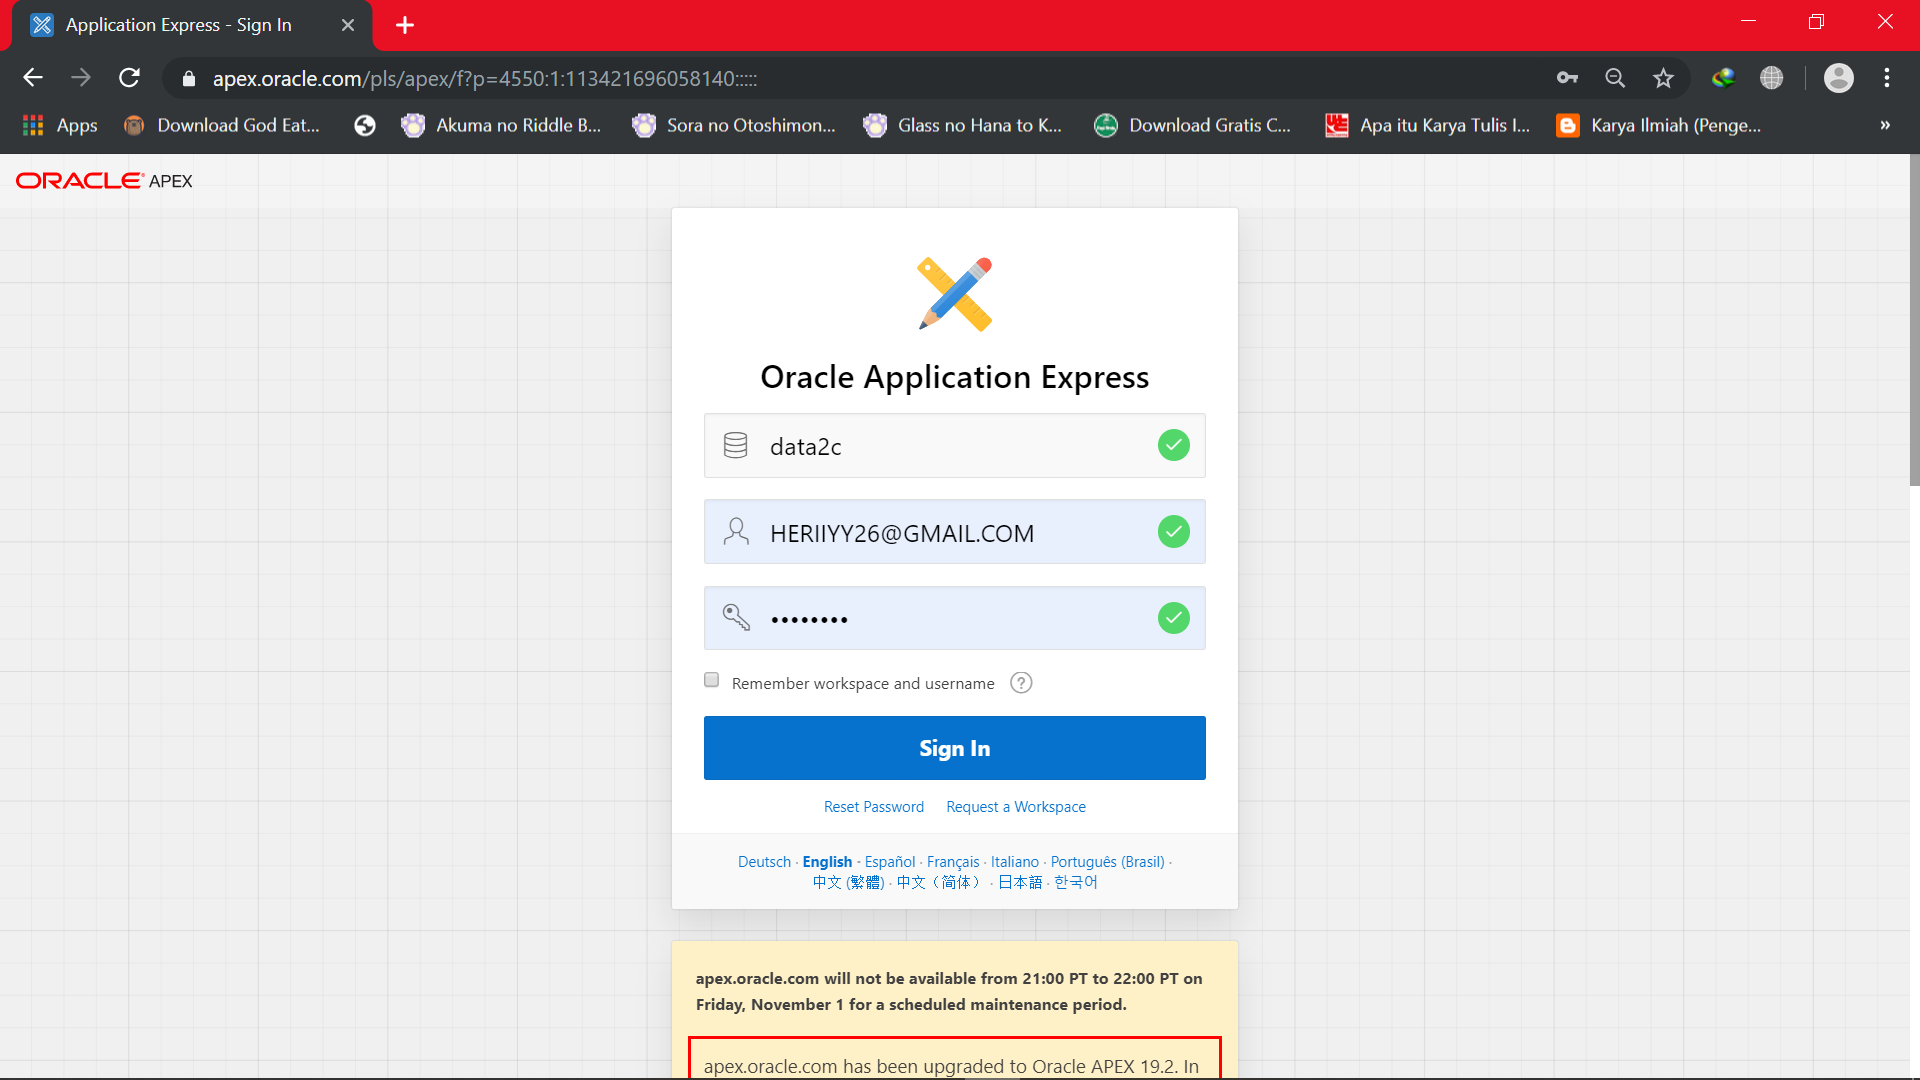
\includegraphics[width=10cm]{figures/Screenshot_1.png}
	\caption{Login}
\end{figure}
\item Klik App Builder - Create - From a File 
\begin{figure}[!htbp]
	\centering
	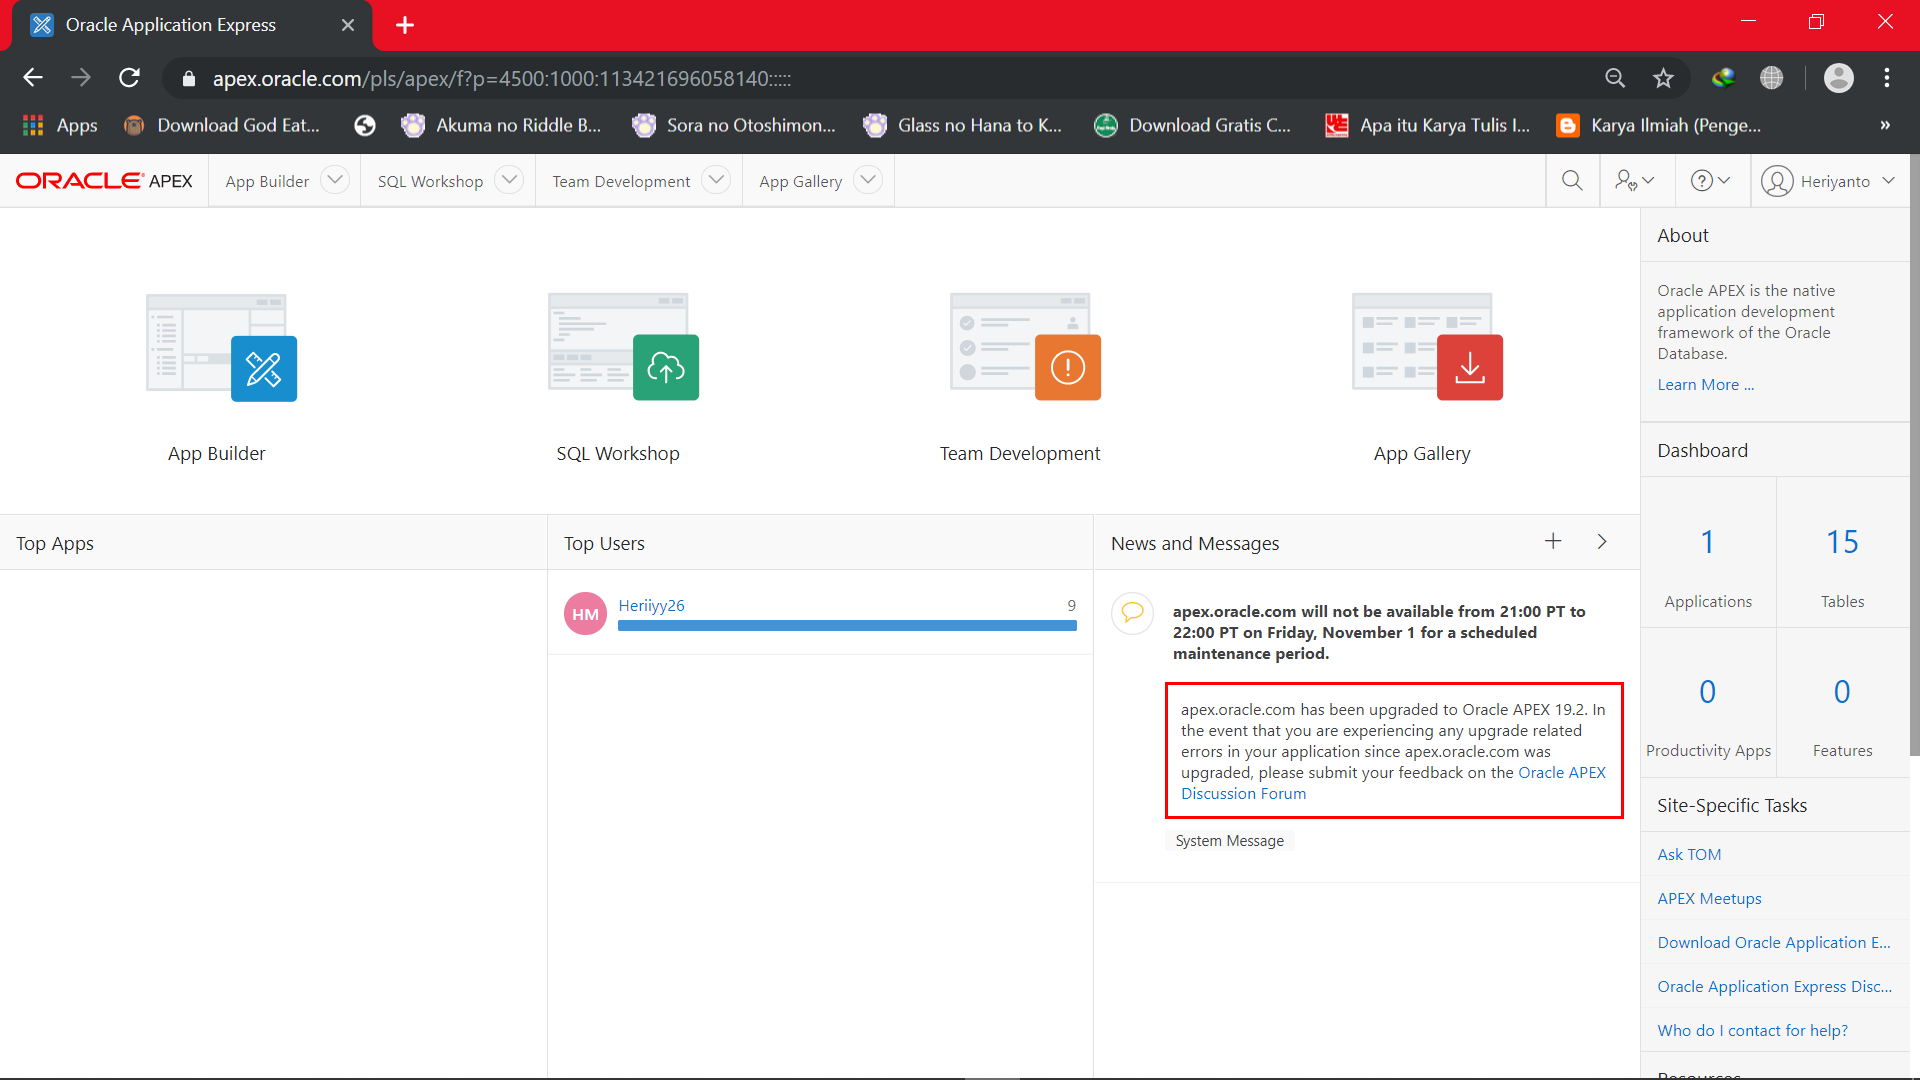
\includegraphics[width=12cm]{figures/Screenshot_2.png}
	\caption{Create Application}
\end{figure}
\item Pilih Copy and Paste dan dari kotak "-Select Sample-" pilih "Movies" lalu klik "Next"
\begin{figure}[!htpb]
	\centering
	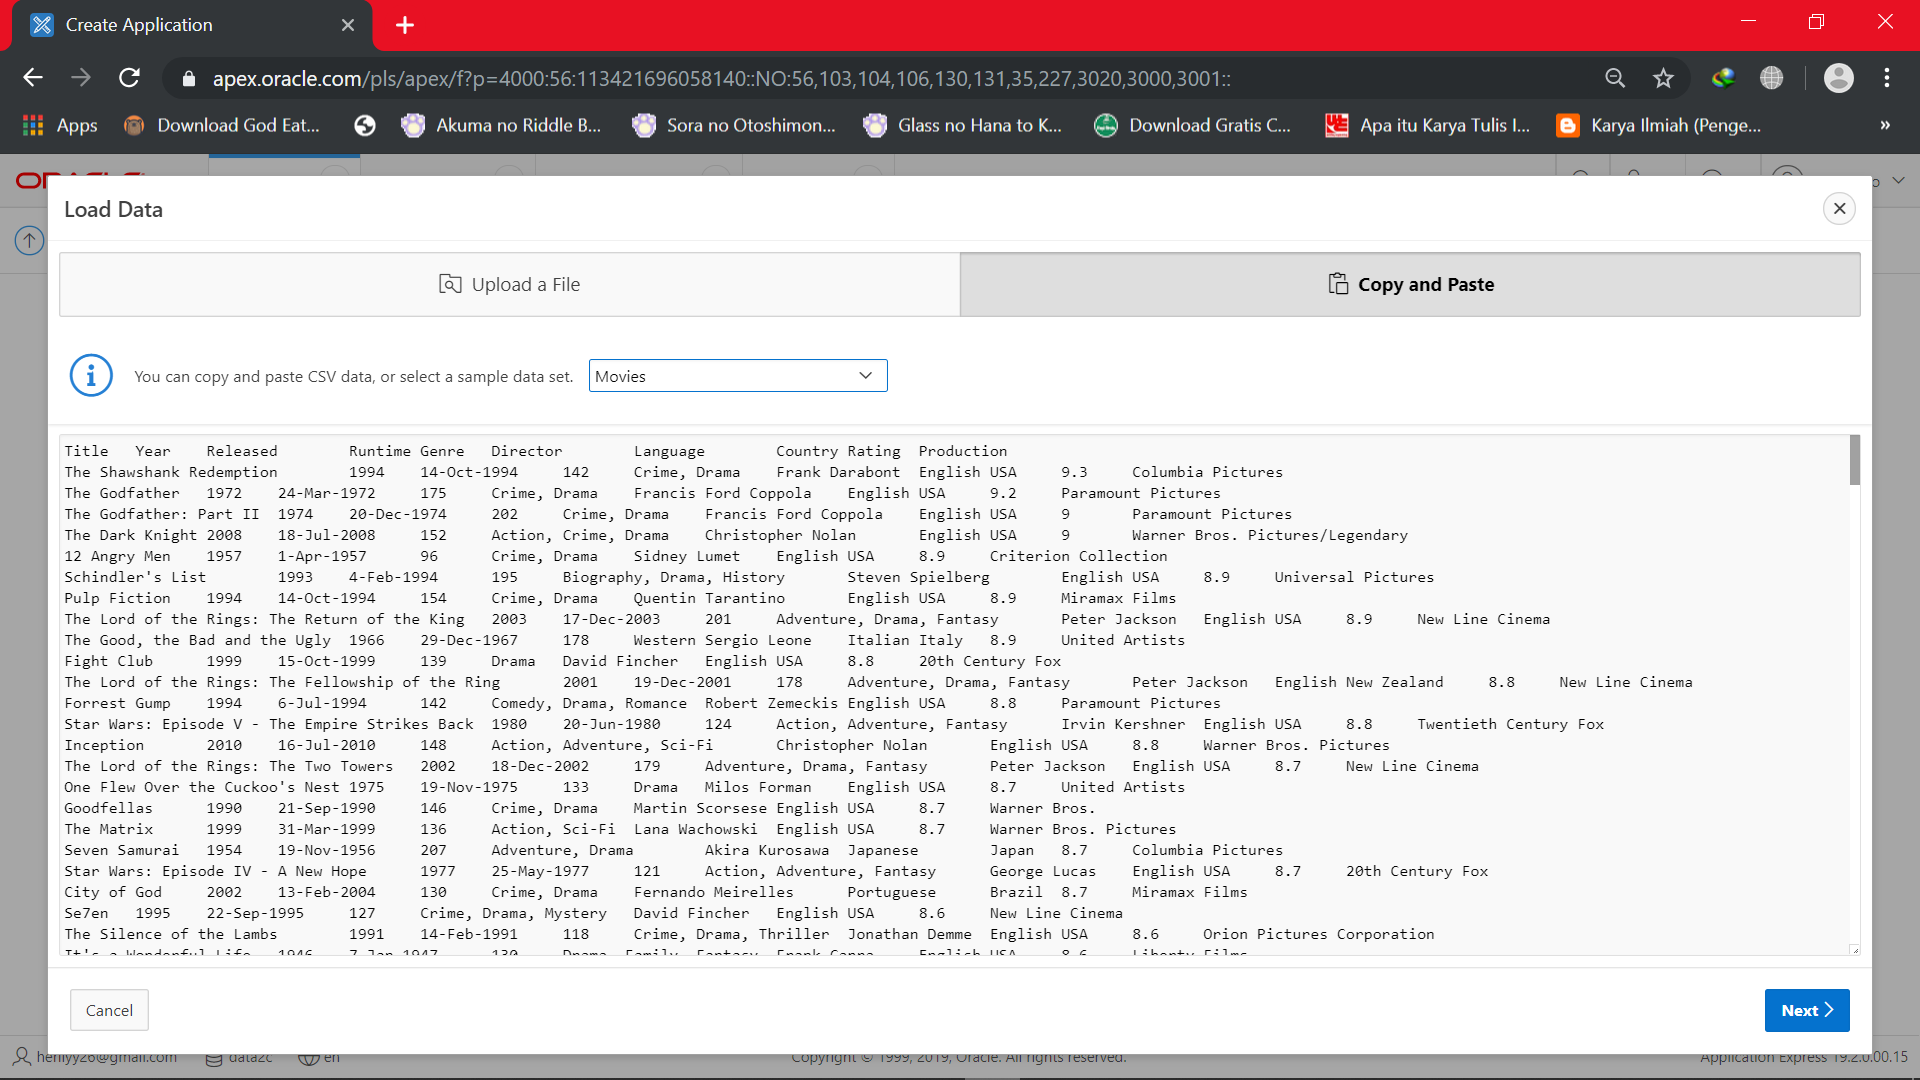
\includegraphics[width=12cm]{figures/Screenshot_3.png}
	\caption{Create Application}
\end{figure}
\item Masukkan tabel name dengan nama MOVIES lalu klik Load Data dan tunggu sampai proses selesai.
\begin{figure}[!htpb]
	\centering
	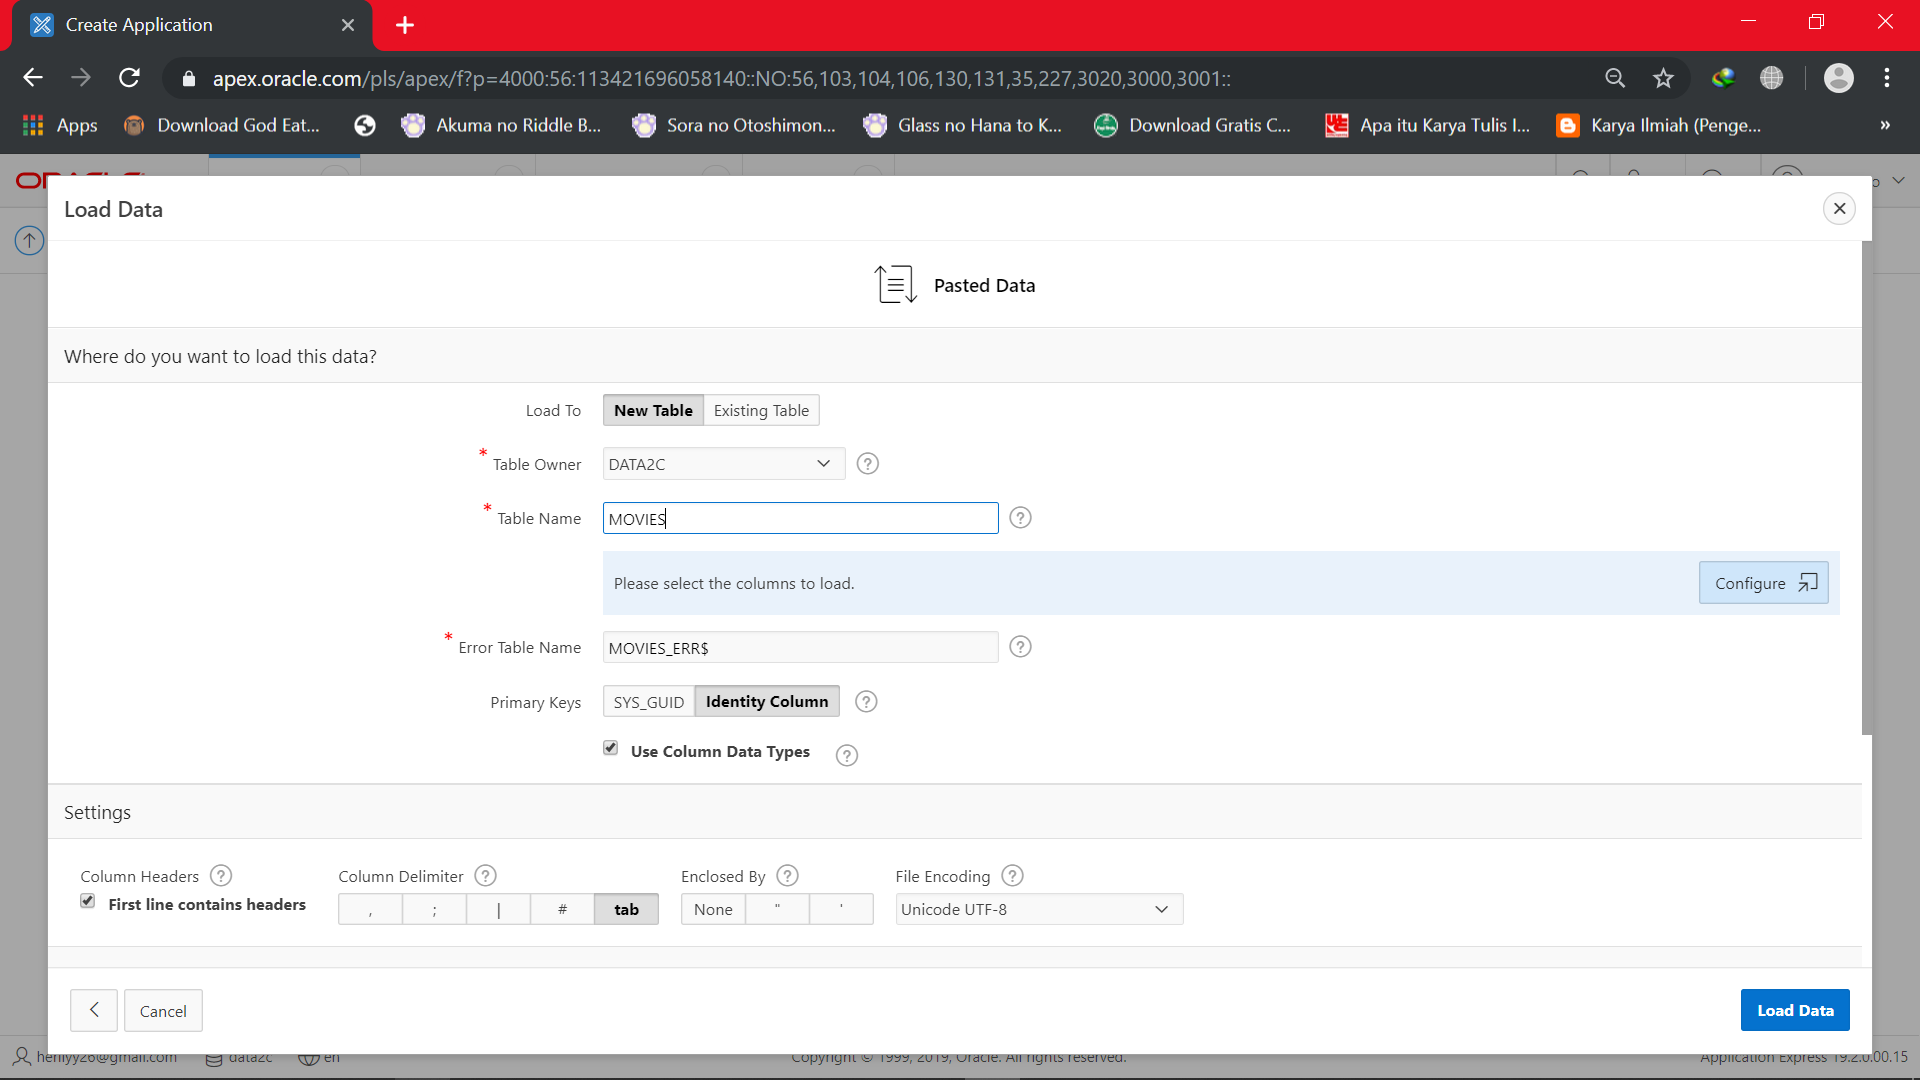
\includegraphics[width=12cm]{figures/Screenshot_4.png}
	\caption{Create Application}
\end{figure}
\item Lalu klik Create Application
\begin{figure}[!htpb]
	\centering
	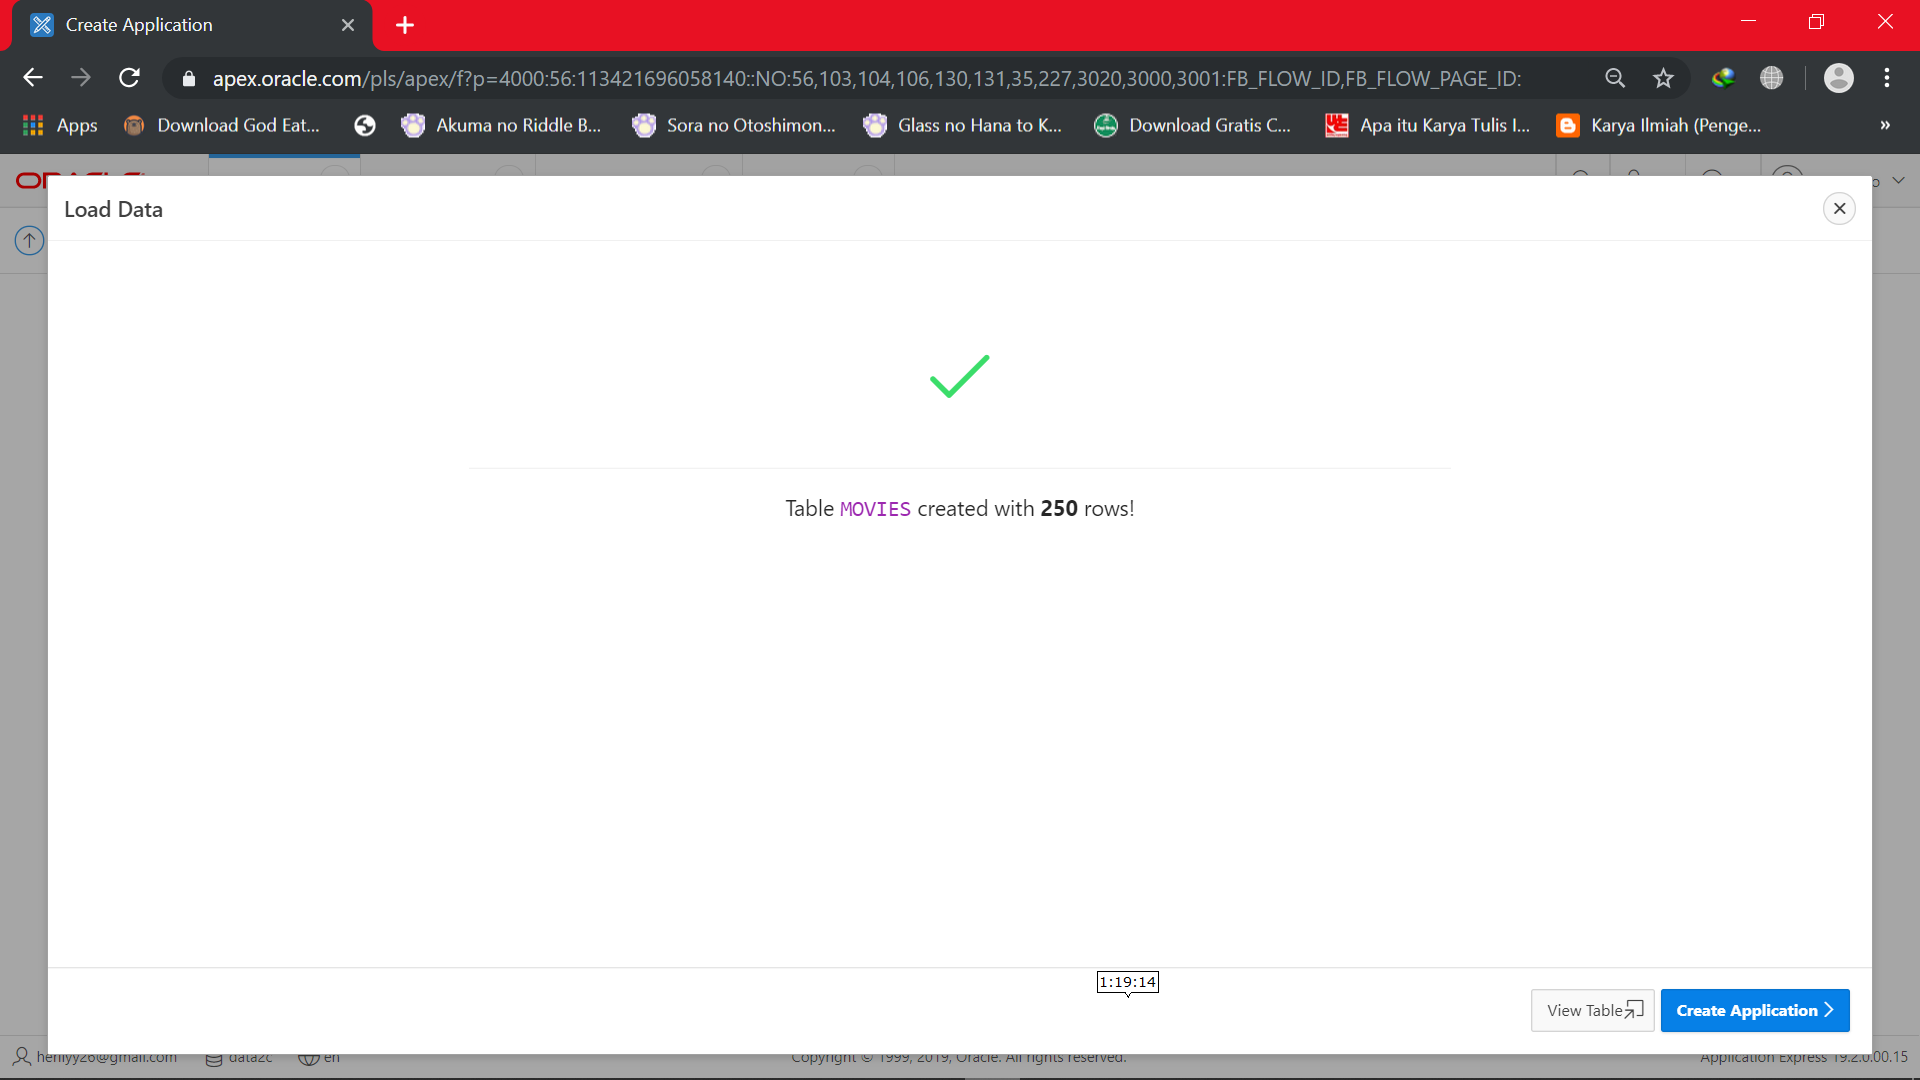
\includegraphics[width=12cm]{figures/Screenshot_5.png}
	\caption{Create Application}
\end{figure}
\item Scroll ke bawah dan pilih "Check all" lalu Klik "Create Application". Tunggu proses sampai selesai.
\begin{figure}[!htpb]
	\centering
	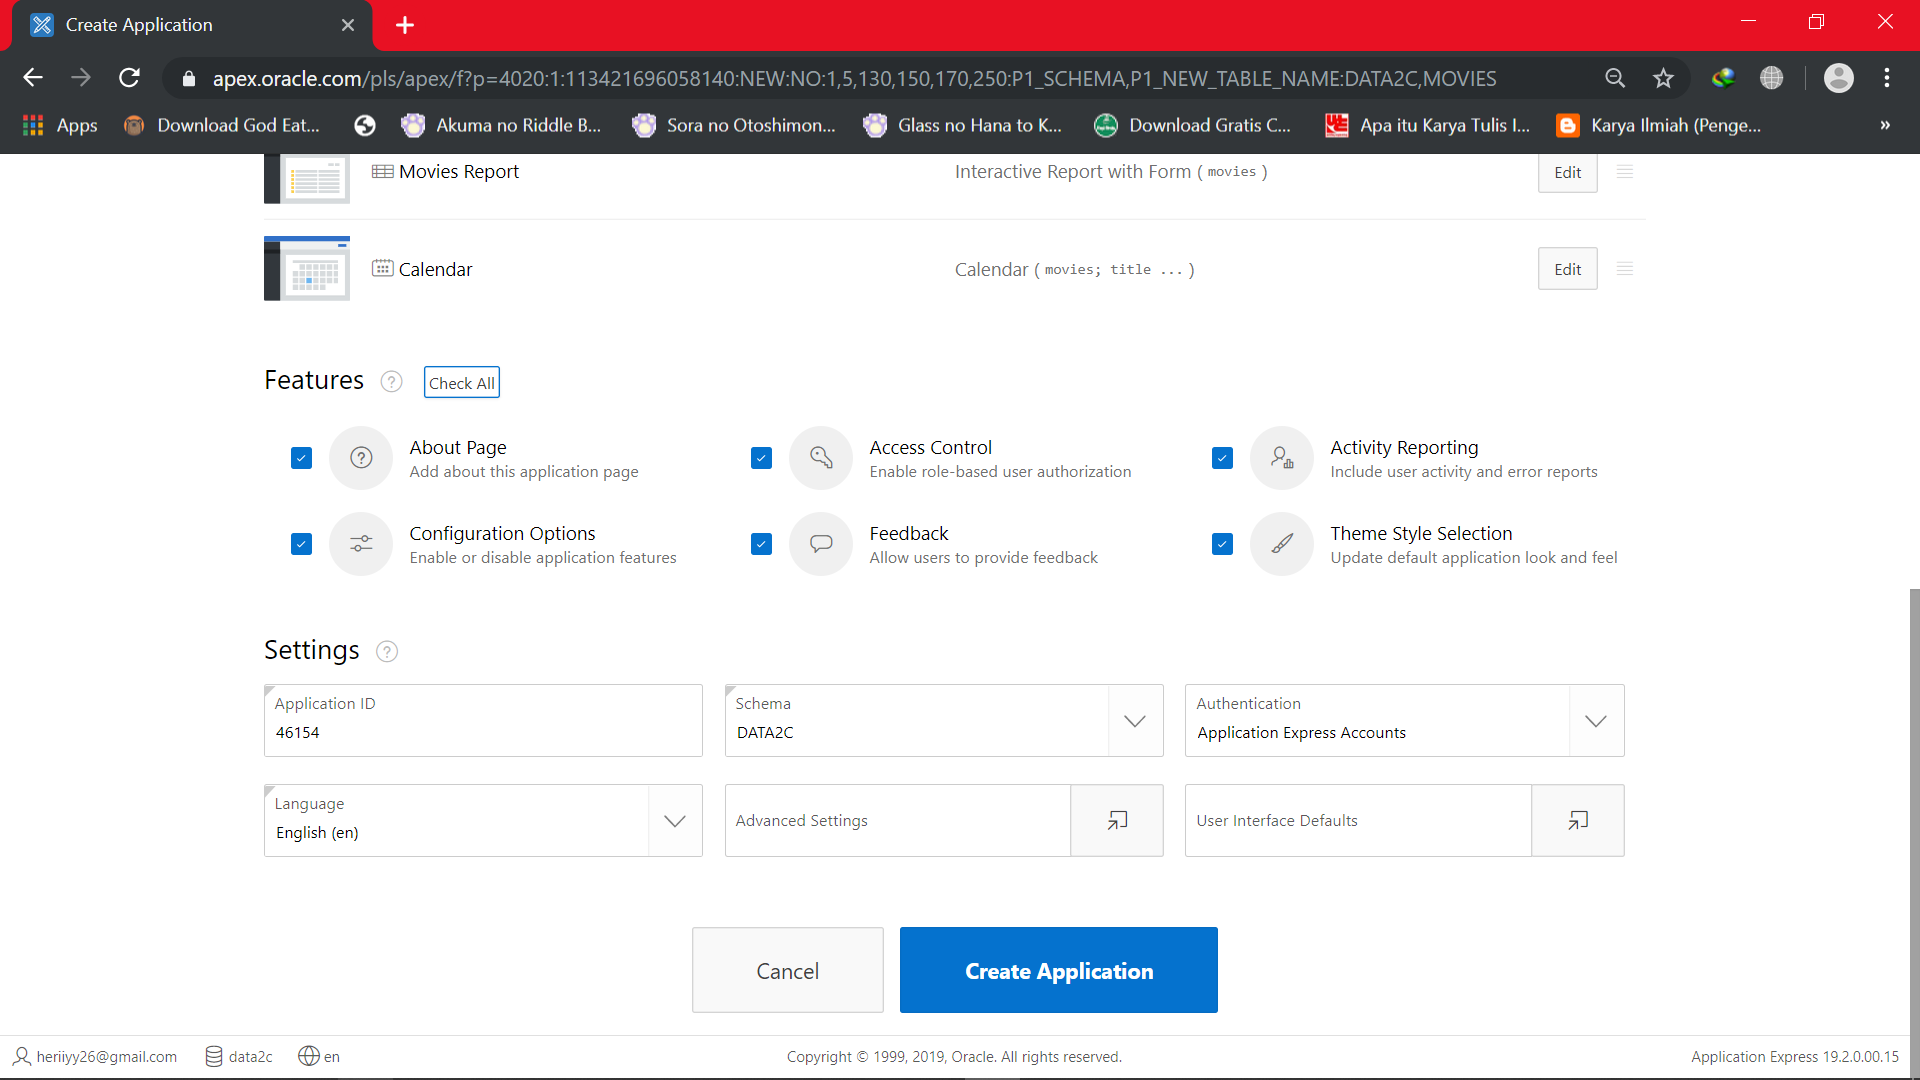
\includegraphics[width=12cm]{figures/Screenshot_6.png}
	\caption{Create Application}
\end{figure}
\item Aplikasi telah selesai dan siap dijalankan klik "Run Application".
\begin{figure}[!htpb]
	\centering
	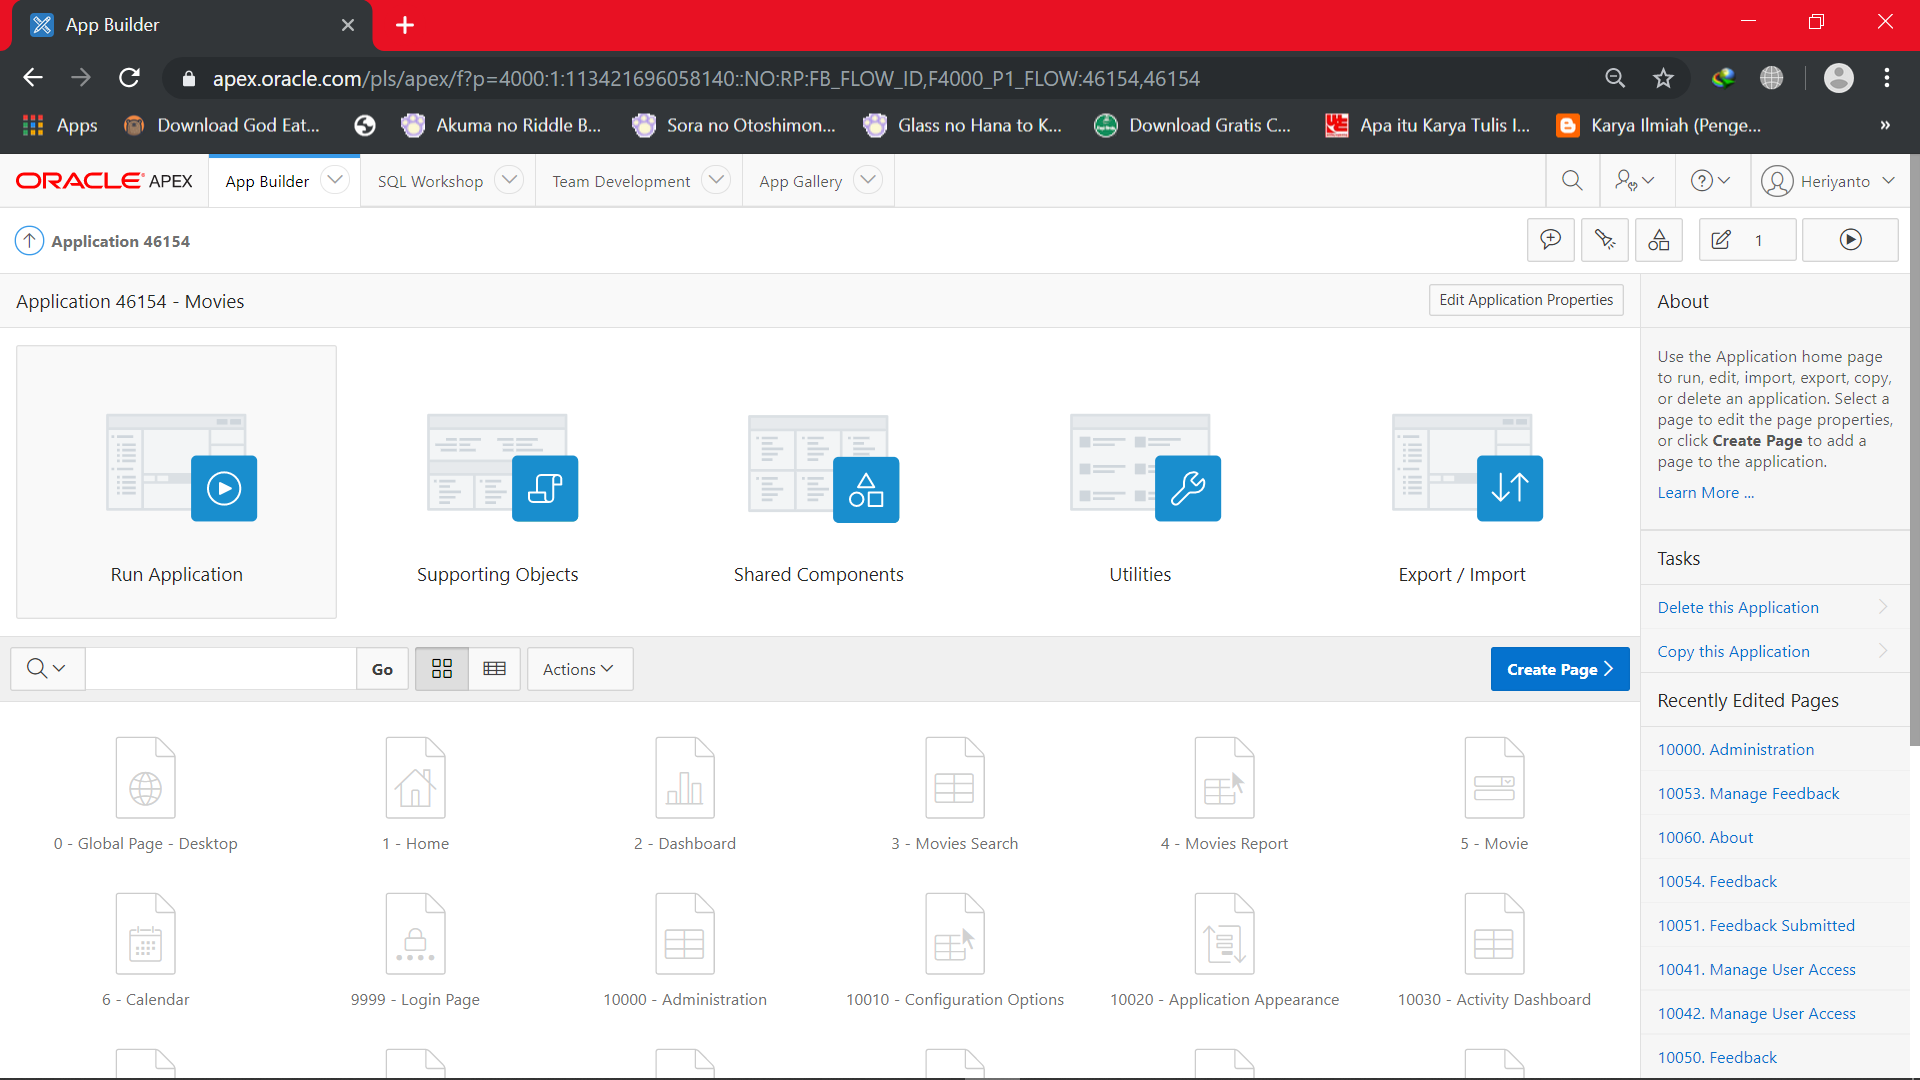
\includegraphics[width=12cm]{figures/Screenshot_7.png}
	\caption{Create Application}
\end{figure}
\item Silahkan login untuk masuk ke aplikasi.
\begin{figure}[!htpb]
	\centering
	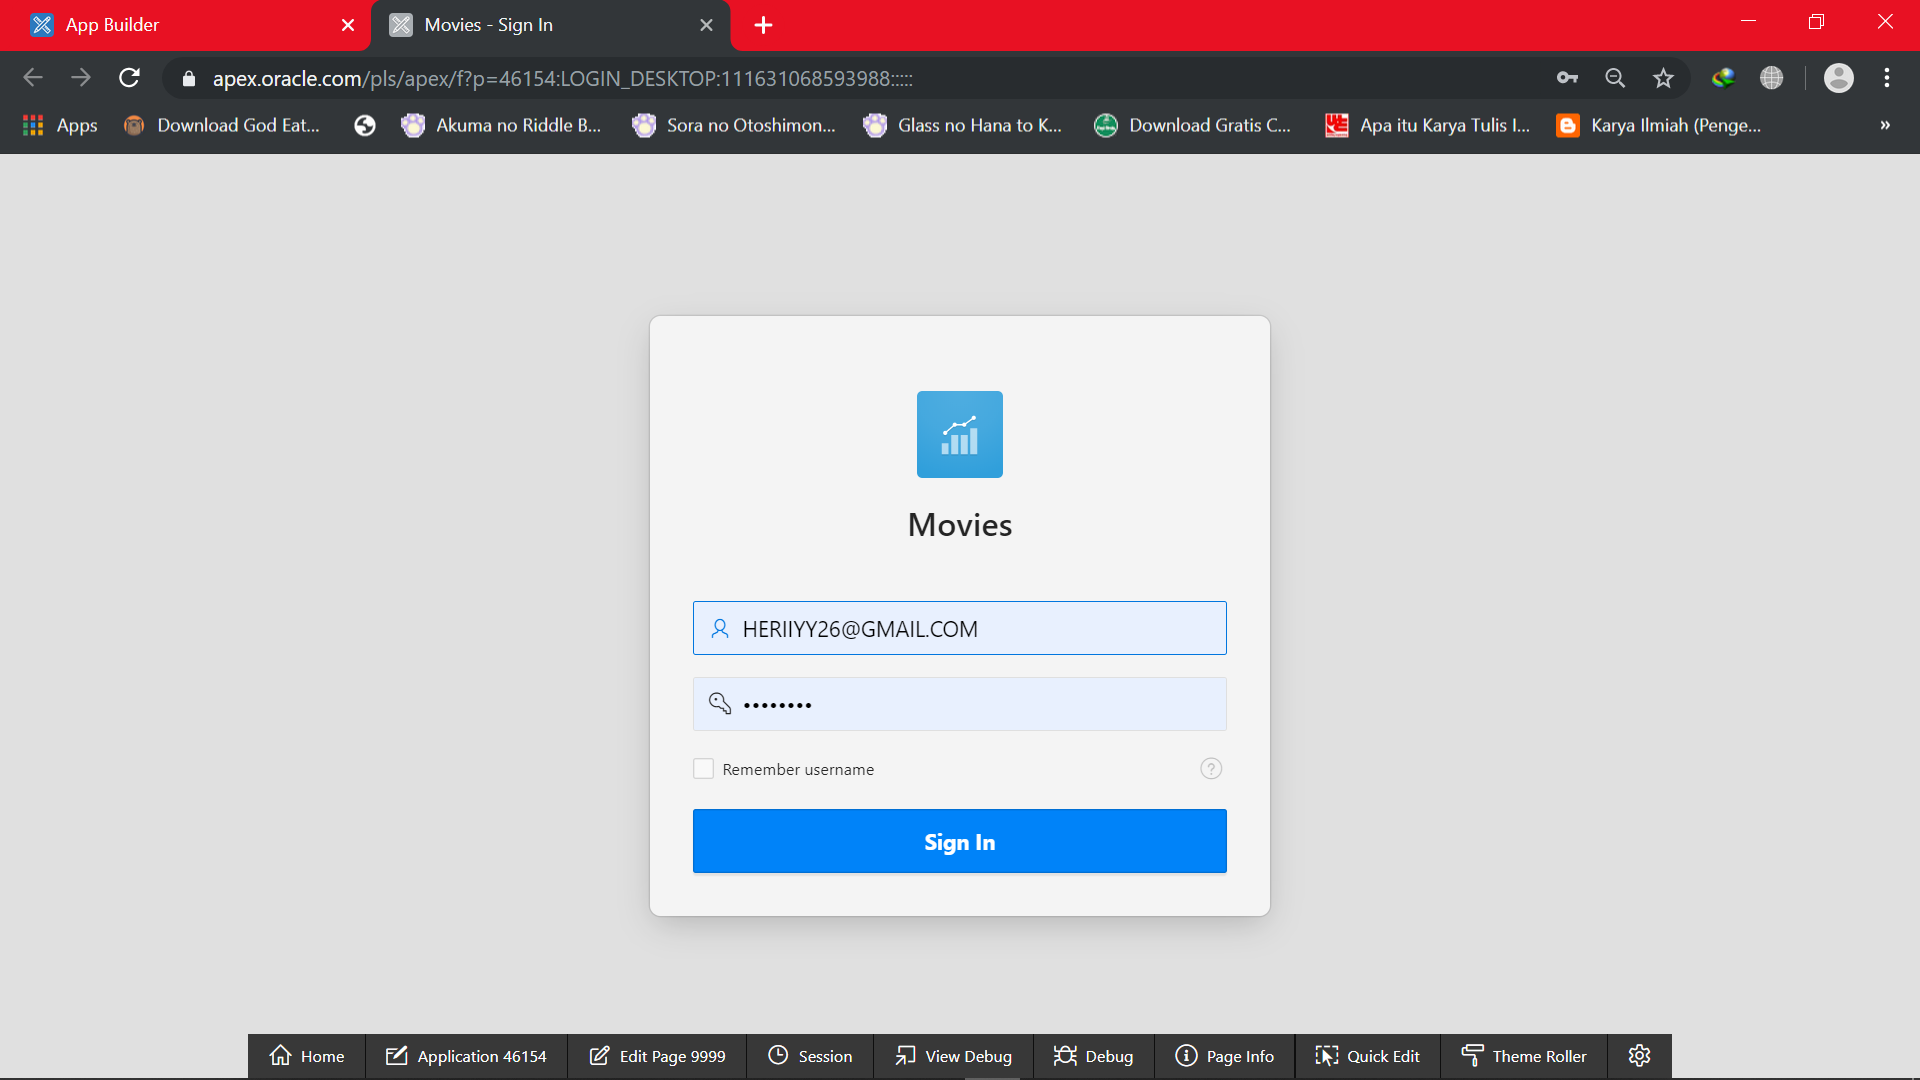
\includegraphics[width=12cm]{figures/Screenshot_8.png}
	\caption{Movies Application}
\end{figure}
\item Tampilan Utama dari Movies Application, silahkan klik menu-menu dari aplikasi ini.
\begin{figure}[!htpb]
	\centering
	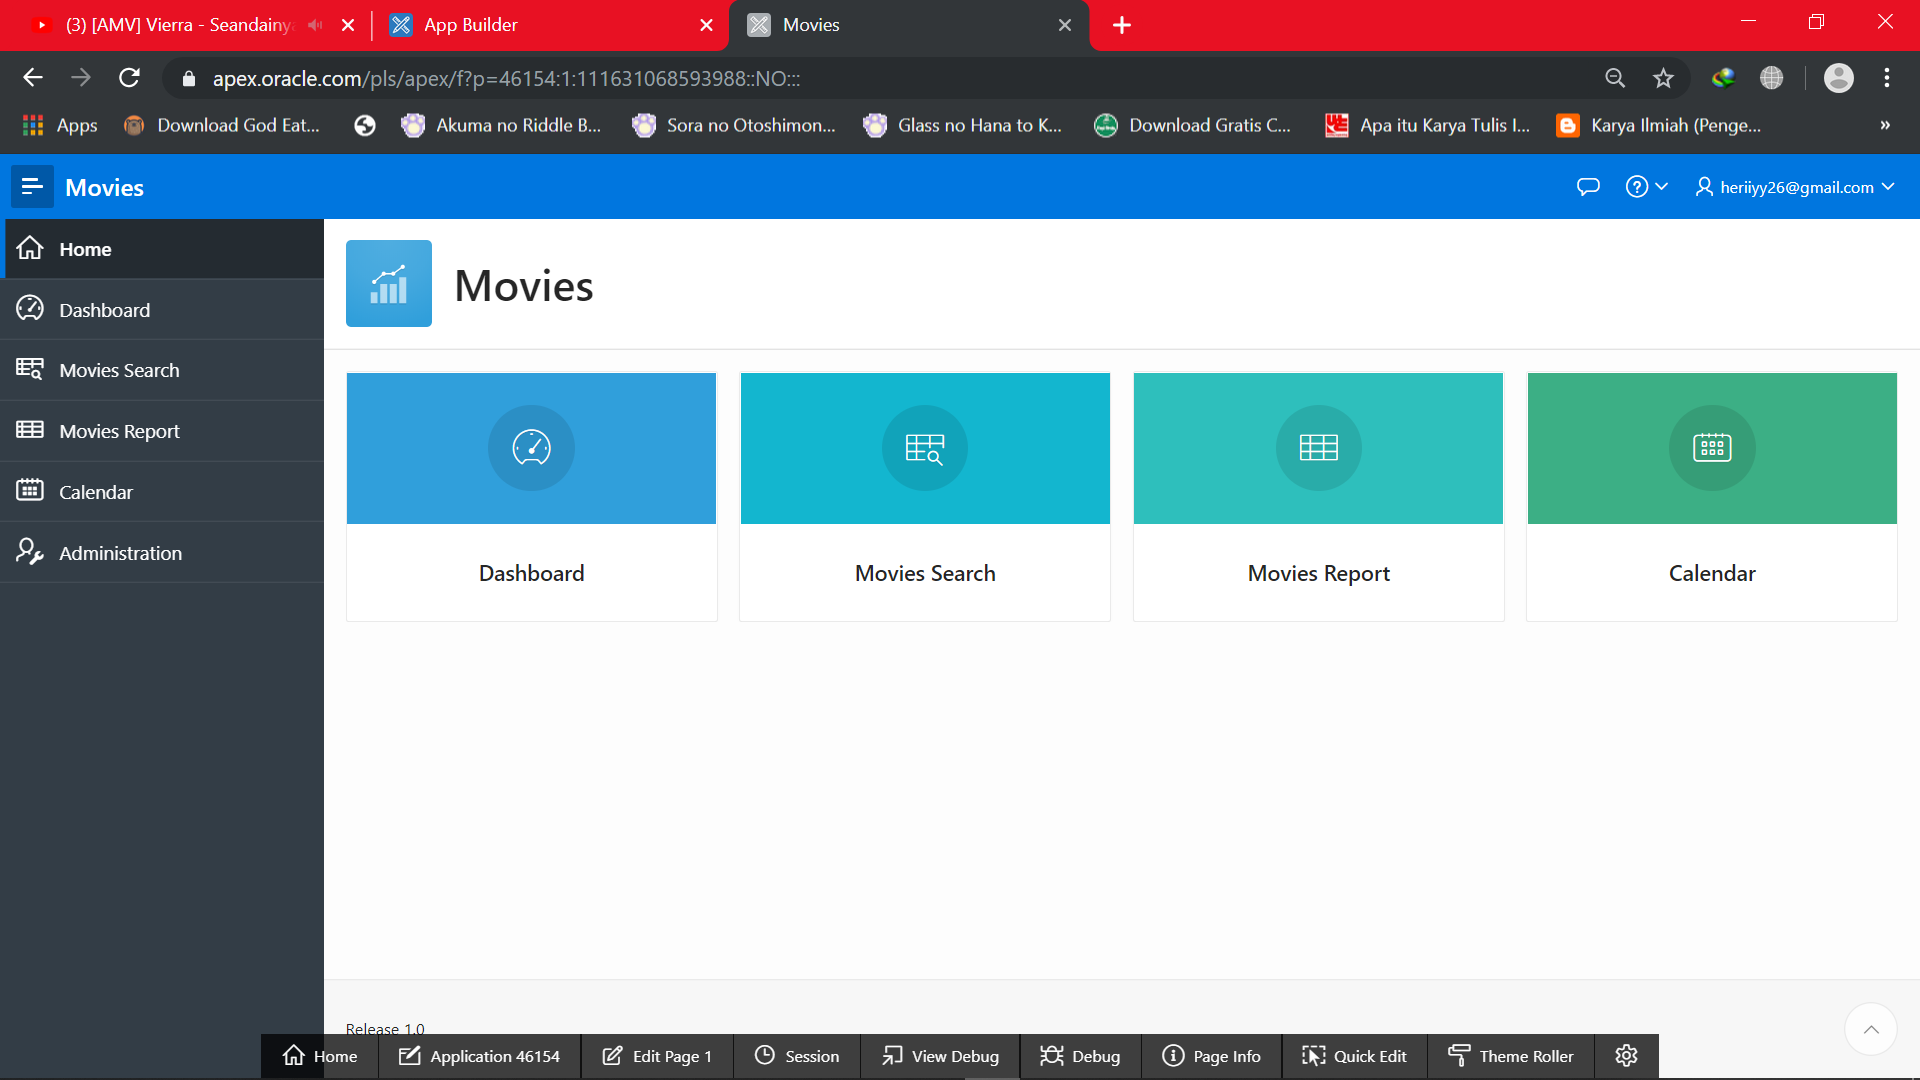
\includegraphics[width=12cm]{figures/Screenshot_9.png}
	\caption{Movies Application}
\end{figure}
\item Mari kita coba mengecek tabel dari movies dengan mengetik sintaks "Select * from movies" di SQL Commands.
\begin{figure}[!htpb]
	\centering
	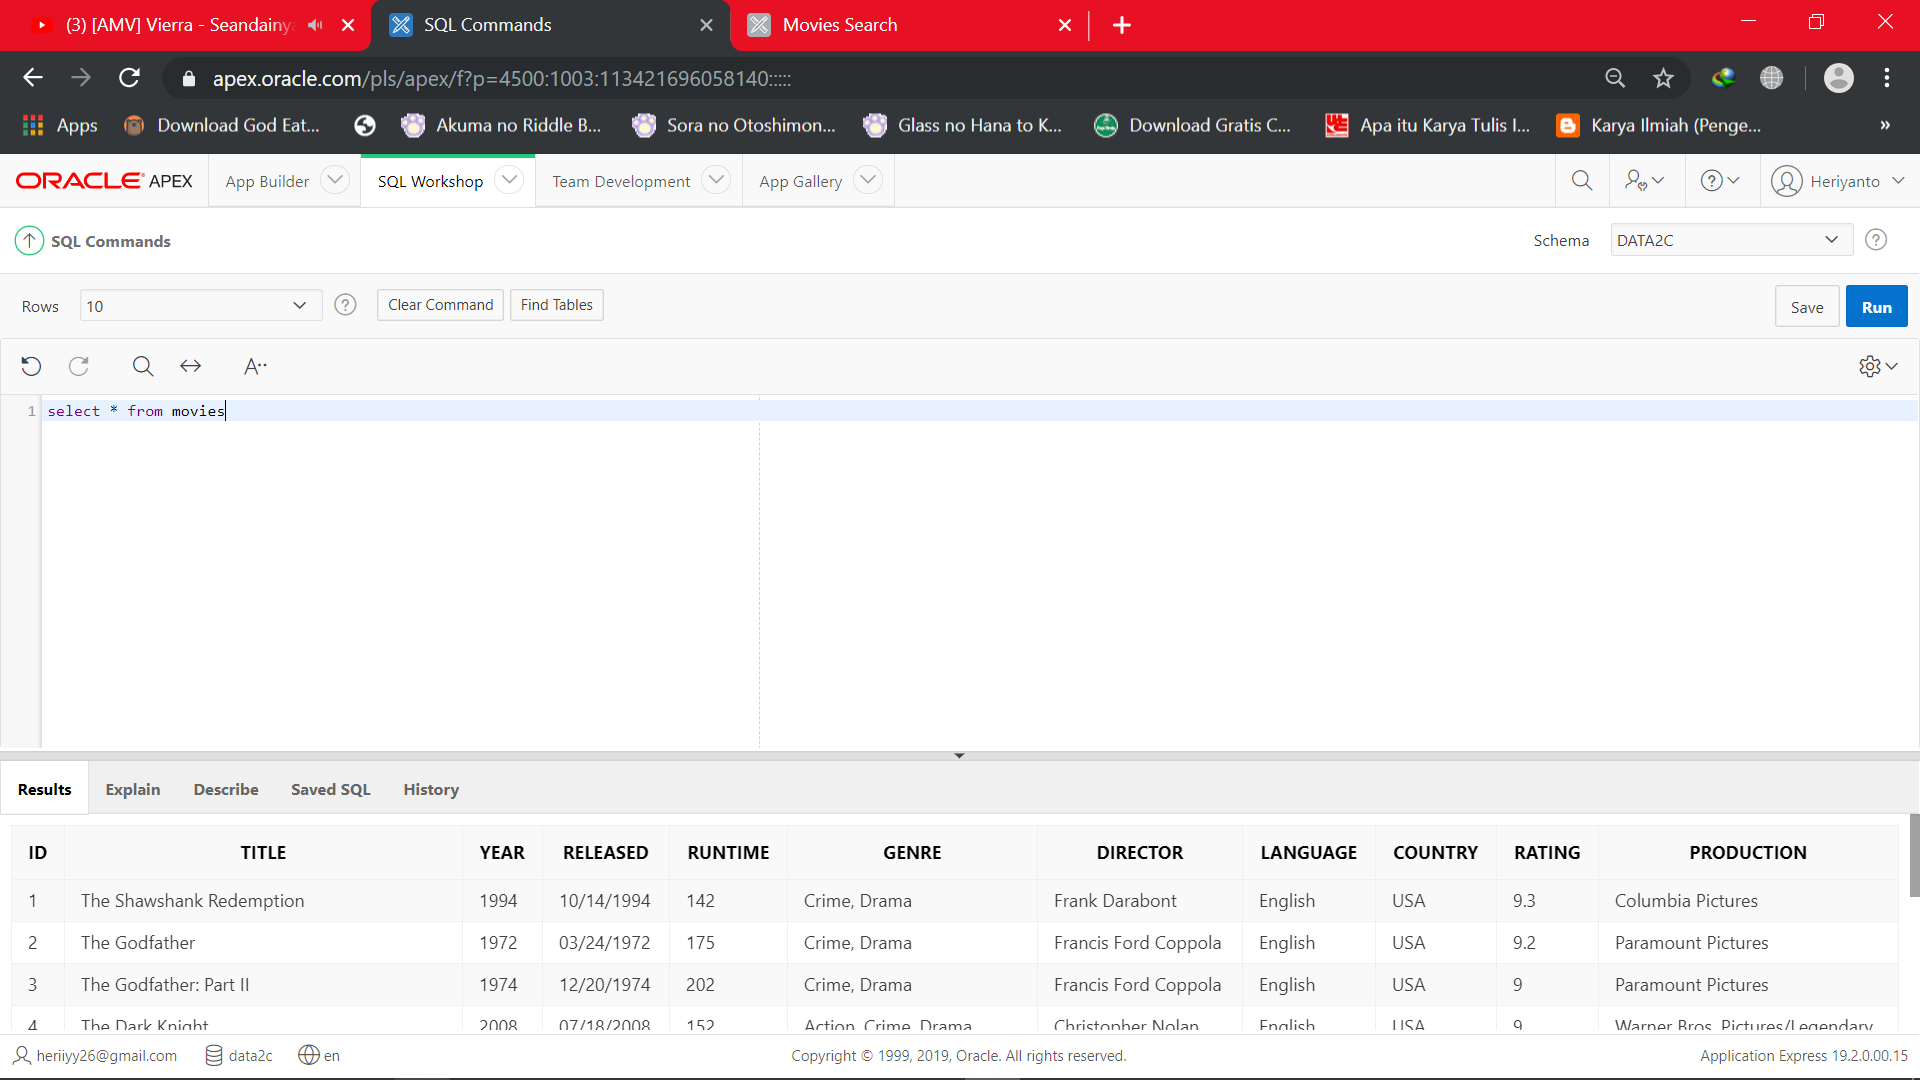
\includegraphics[width=12cm]{figures/Screenshot_10.png}
	\caption{Movies Application}
\end{figure}
\end{itemize}
\section{Quick SQL}
Quick SQL pada dasarnya adalah bahasa yang dapat Anda gunakan untuk menghasilkan kode SQL yang benar secara sistematis yang dapat Anda gunakan untuk mendesain database dan diimplementasikan dengan sangat cepat dari membuat tabel dan semua yang anda butuhkan untuk membuat aplikasi database dengan tabel dan semua tabel itu akan di Generate.\\
Use Cases:
\begin{itemize}
\item Dengan cepat membuat model data yang kuat
\item Mudah menghasilkan data acak
\item mempelajari SQL create table, pilih, masukkan, indeks, trigger, paket PL / SQL, dan lihat sintaks menggunakan contoh yang disediakan  
\end{itemize}
\subsection{Cara Menggunakan Quick SQL}
\begin{itemize}
\item Di Halaman Utama apex oracle, klik tab "SQL Workshop" lalu Pilih "Utilities" dan terakhir Pilih "Quick SQL" lalu akan muncul tampilan seperti di bawah.
\begin{figure}[!htpb]
	\centering
	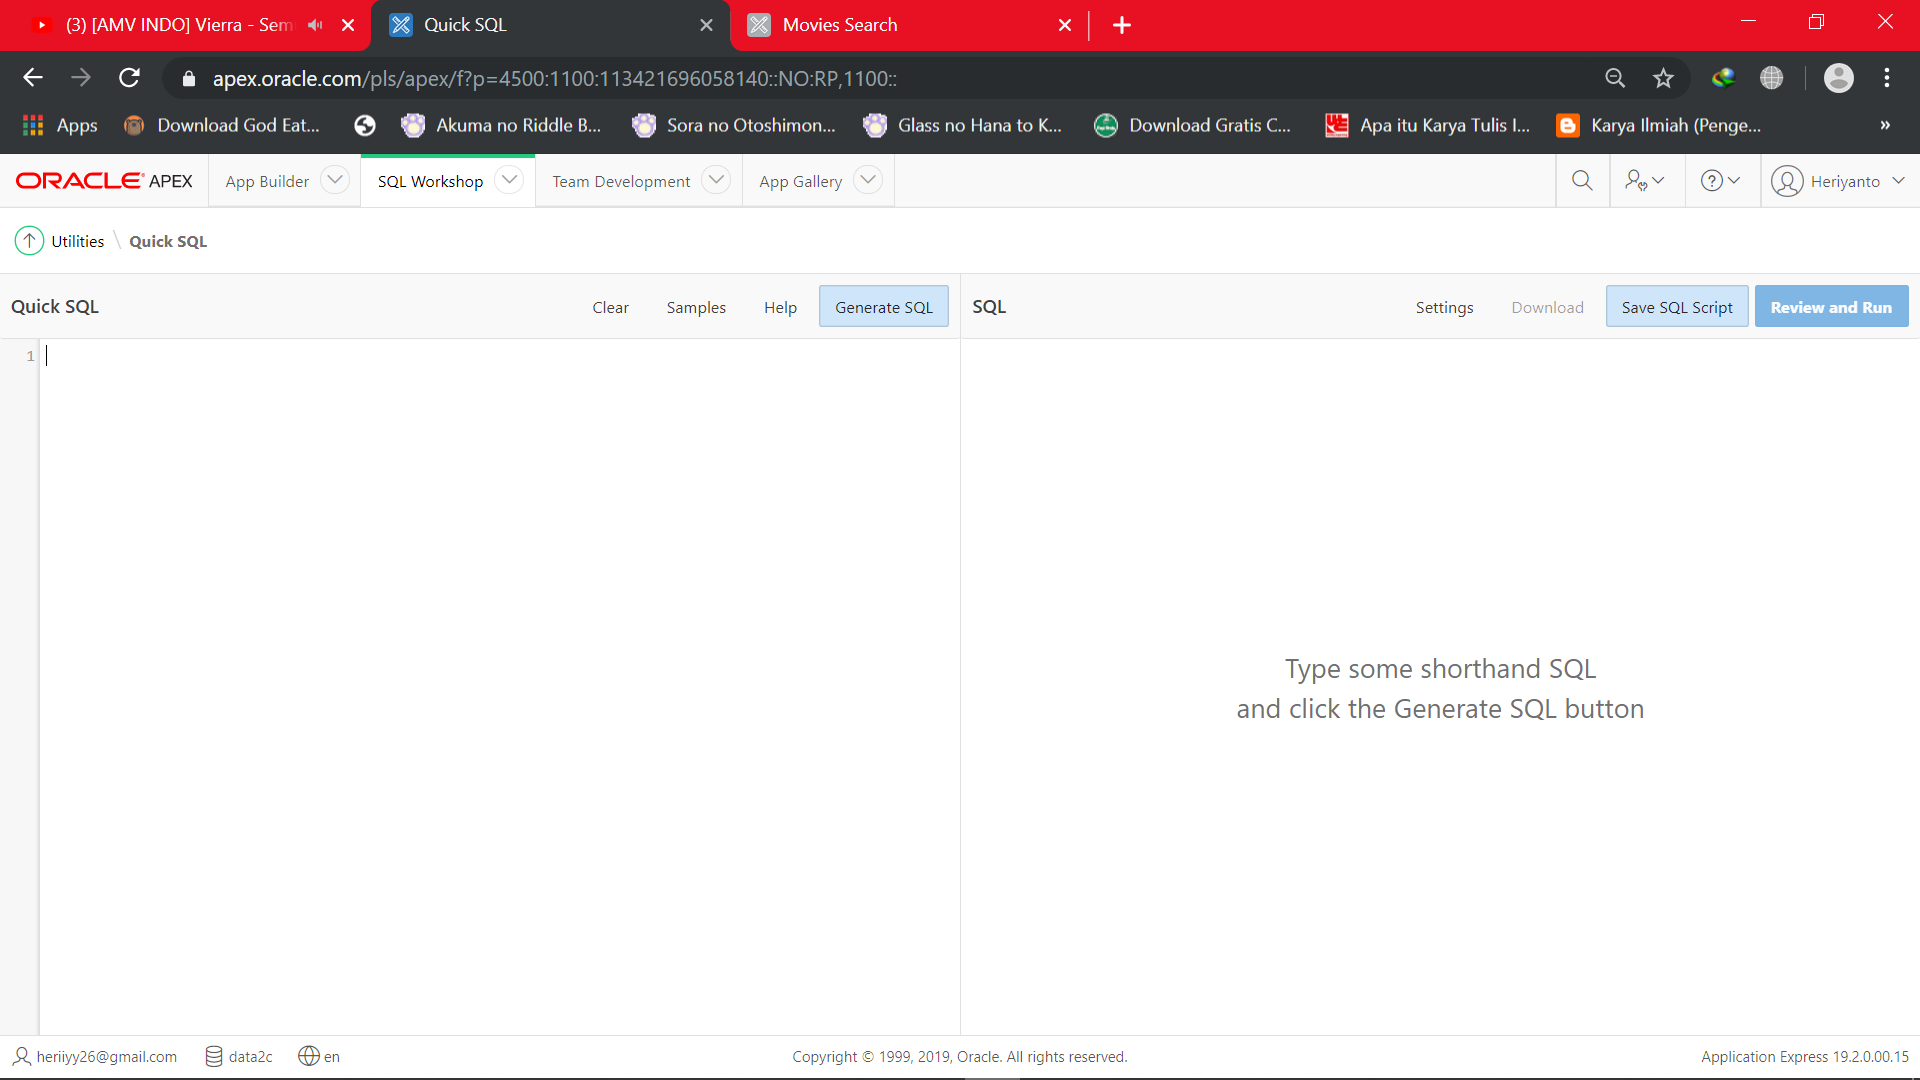
\includegraphics[width=10cm]{figures/Screenshot_11.png}
	\caption{Quick SQL}
\end{figure}
\item Di halaman quick sql Klik "samples", lalu akan muncul tampilan di bawah dan pilih "Load data" pada "Employees Skills".
\begin{figure}[!htpb]
	\centering
	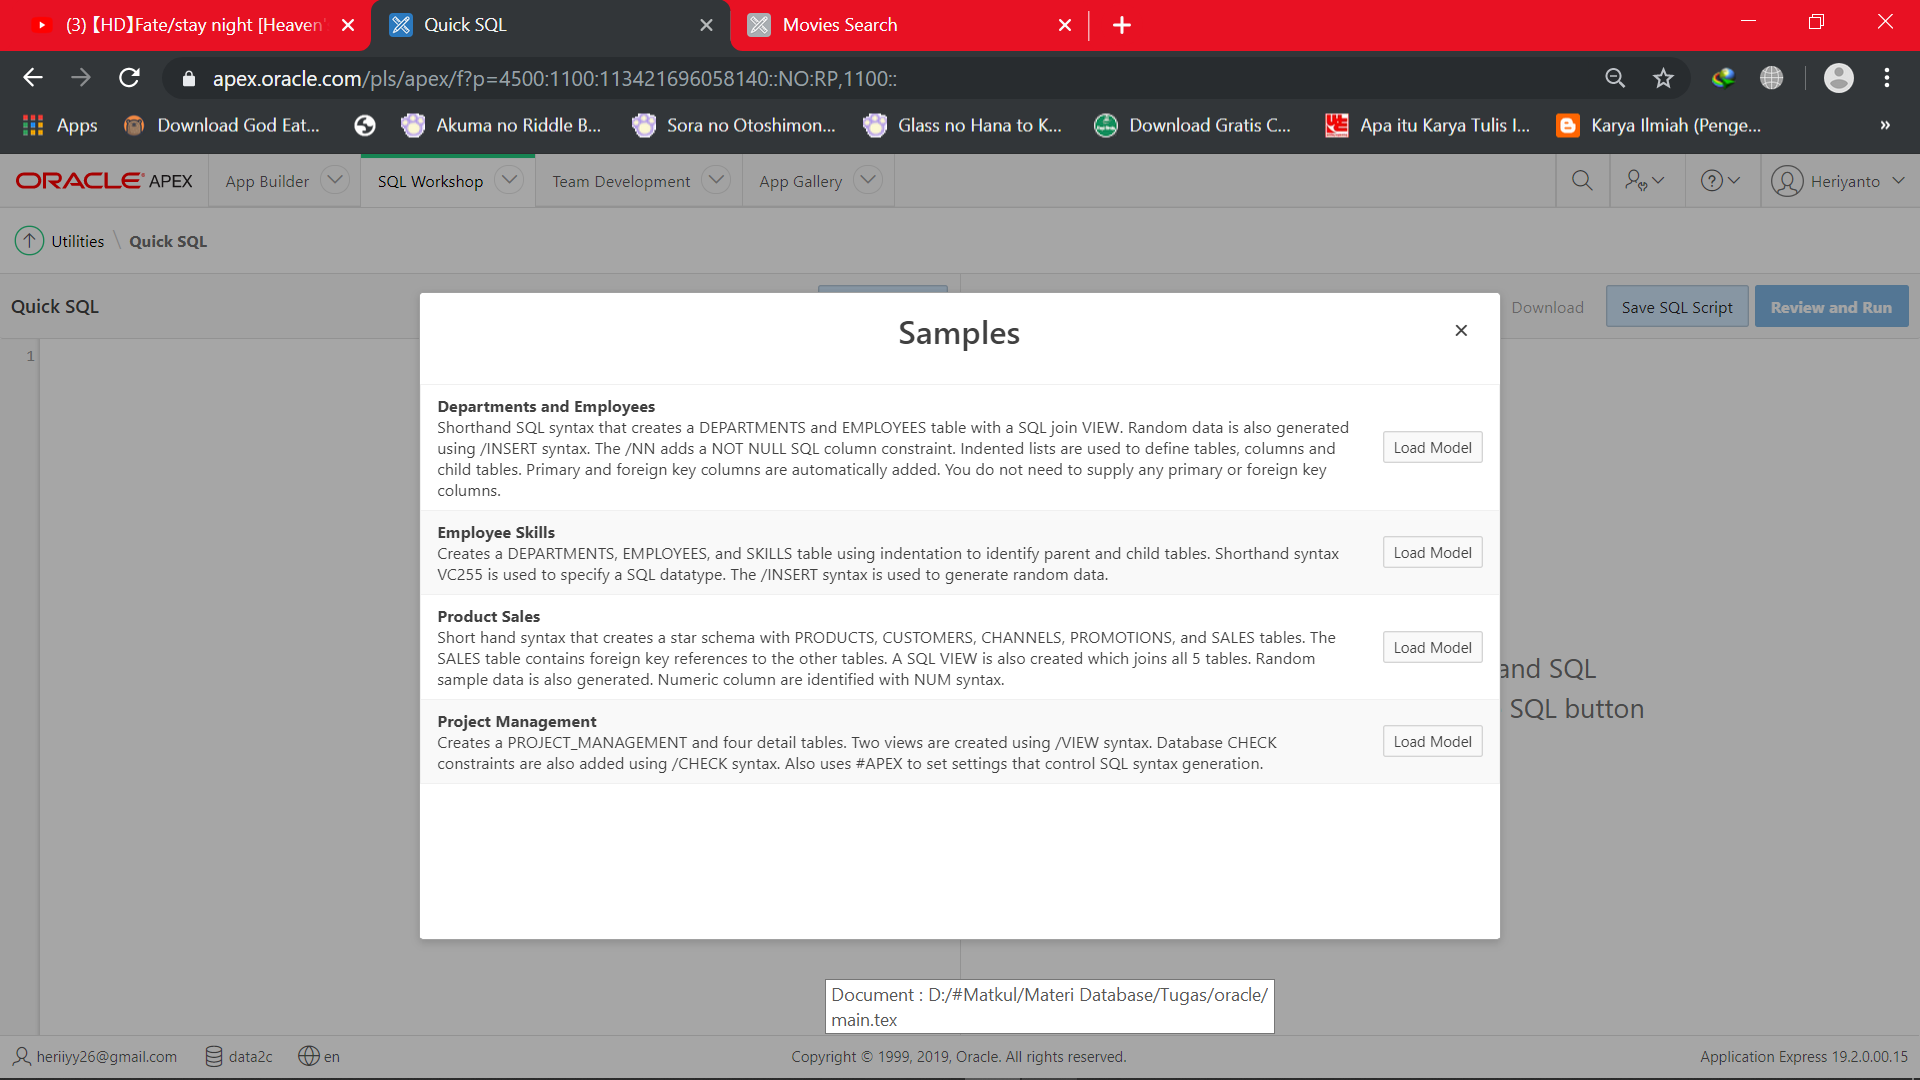
\includegraphics[width=11cm]{figures/Screenshot_12.png}
	\caption{Quick SQL}
\end{figure}
\item Setelah di Load Data akan muncul sintaks seperti di bawah.
\begin{figure}[!htpb]
	\centering
	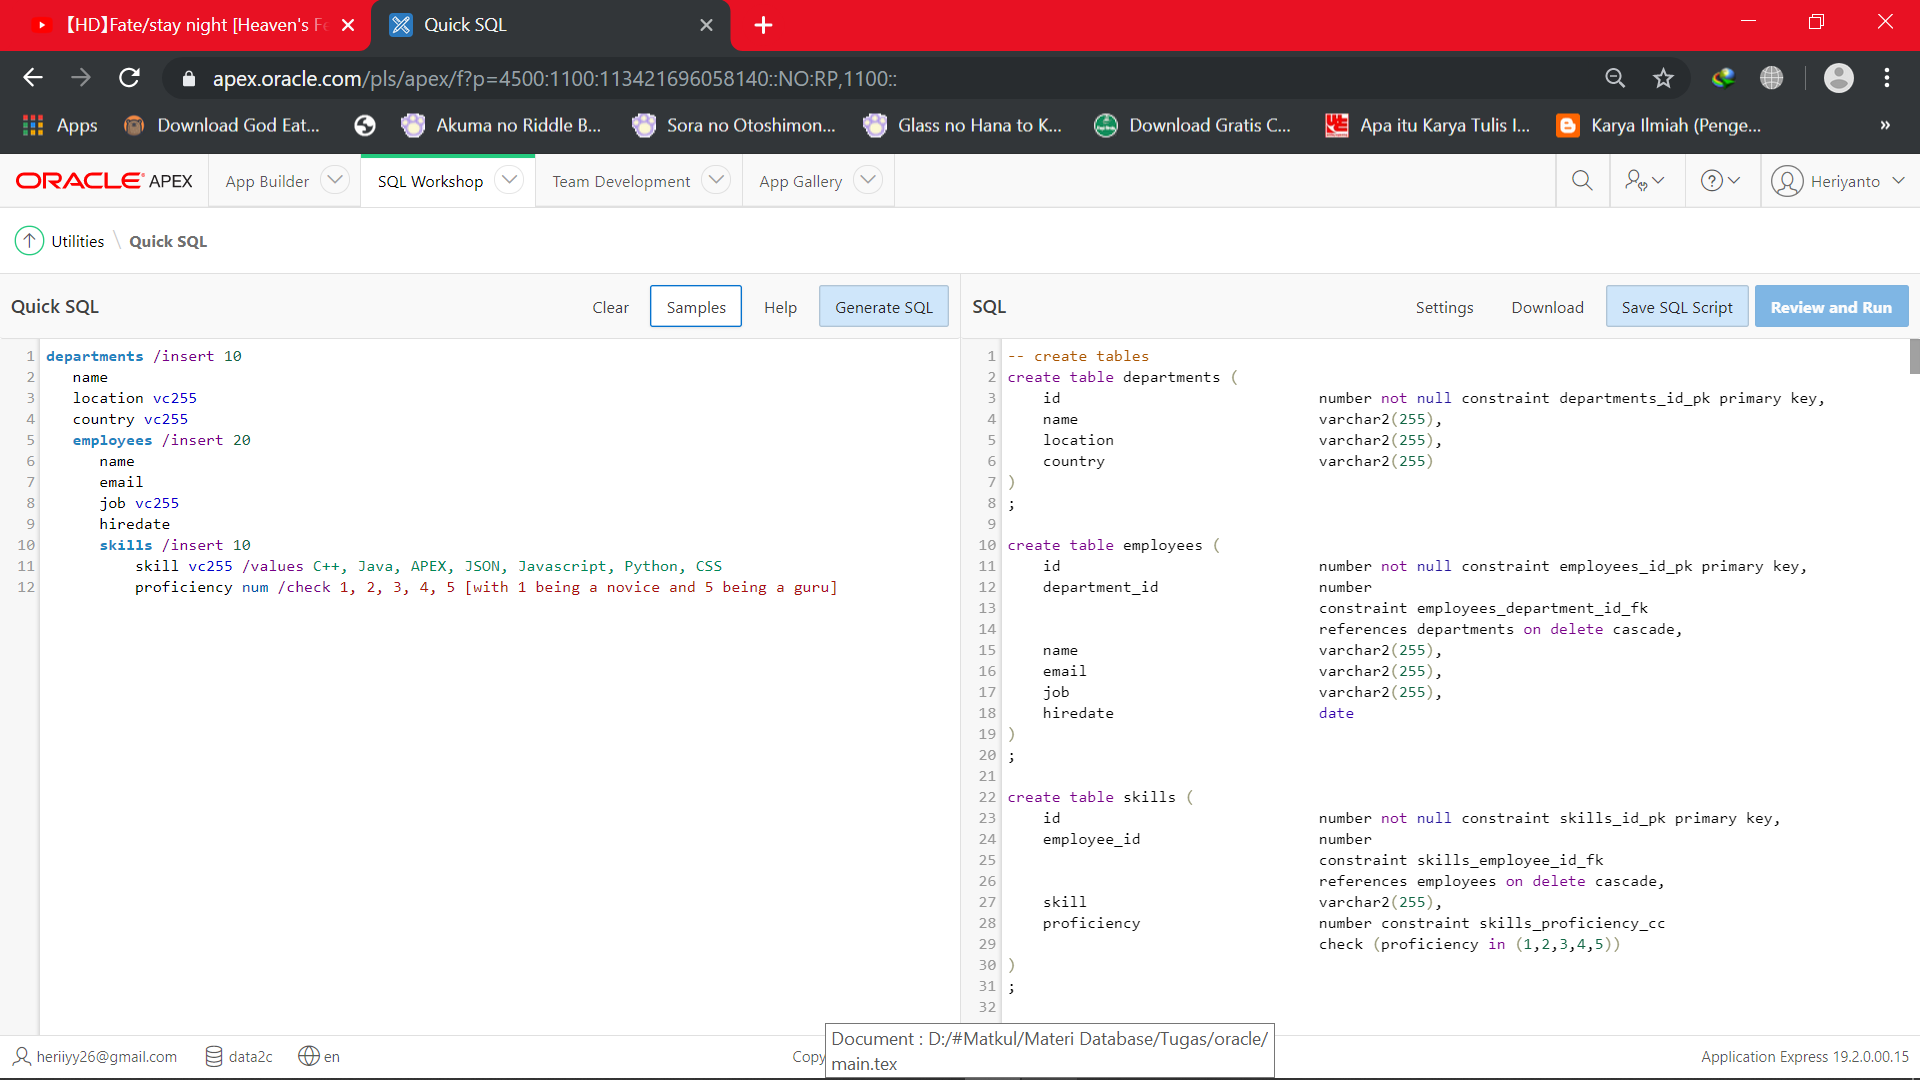
\includegraphics[width=12.5cm]{figures/Screenshot_13.png}
	\caption{Quick SQL}
\end{figure}
\item Pergi ke settings, lalu muncul konfigurasi seperti di bawah.
\begin{figure}[!htpb]
	\centering
	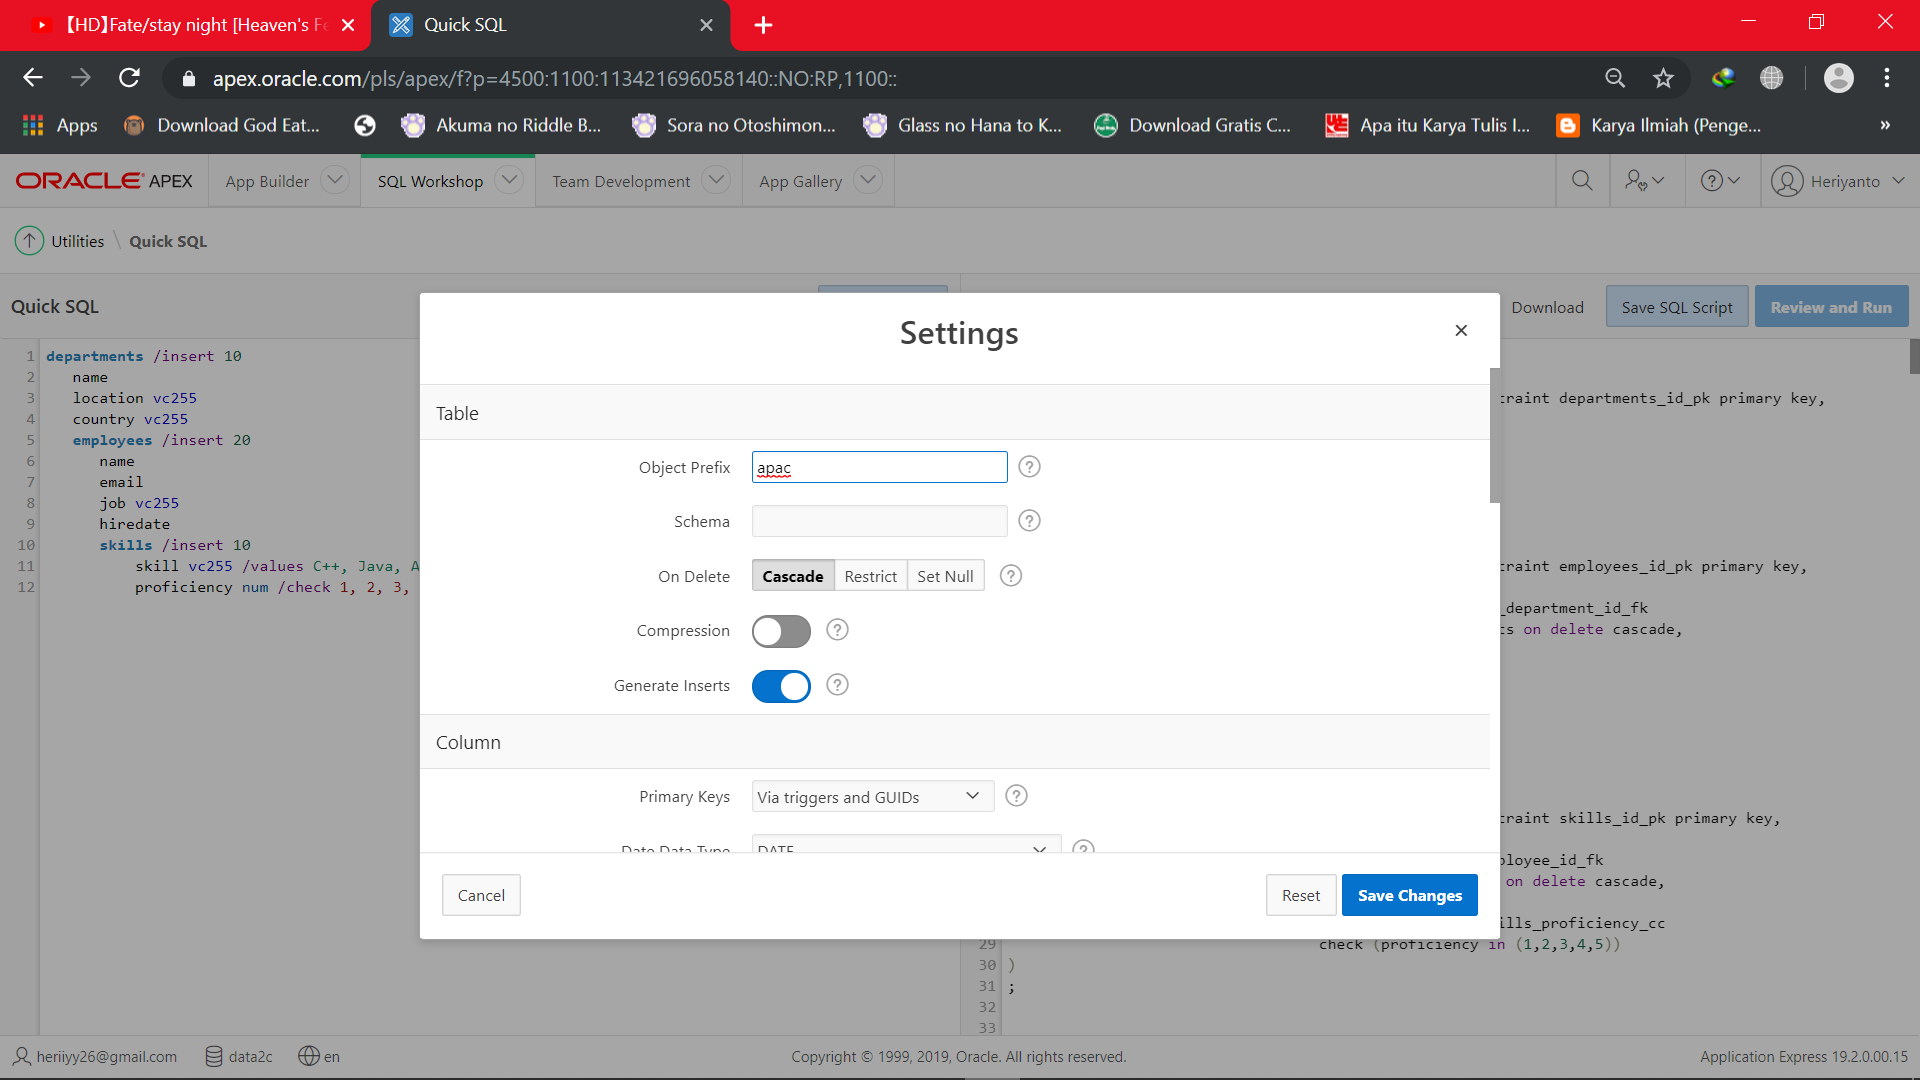
\includegraphics[width=12.5cm]{figures/Screenshot_14.png}
	\caption{Quick SQL}
\end{figure}
\item Scroll ke bawah, cari "Include Drops" lalu centang dan save.
\begin{figure}[!htpb]
	\centering
	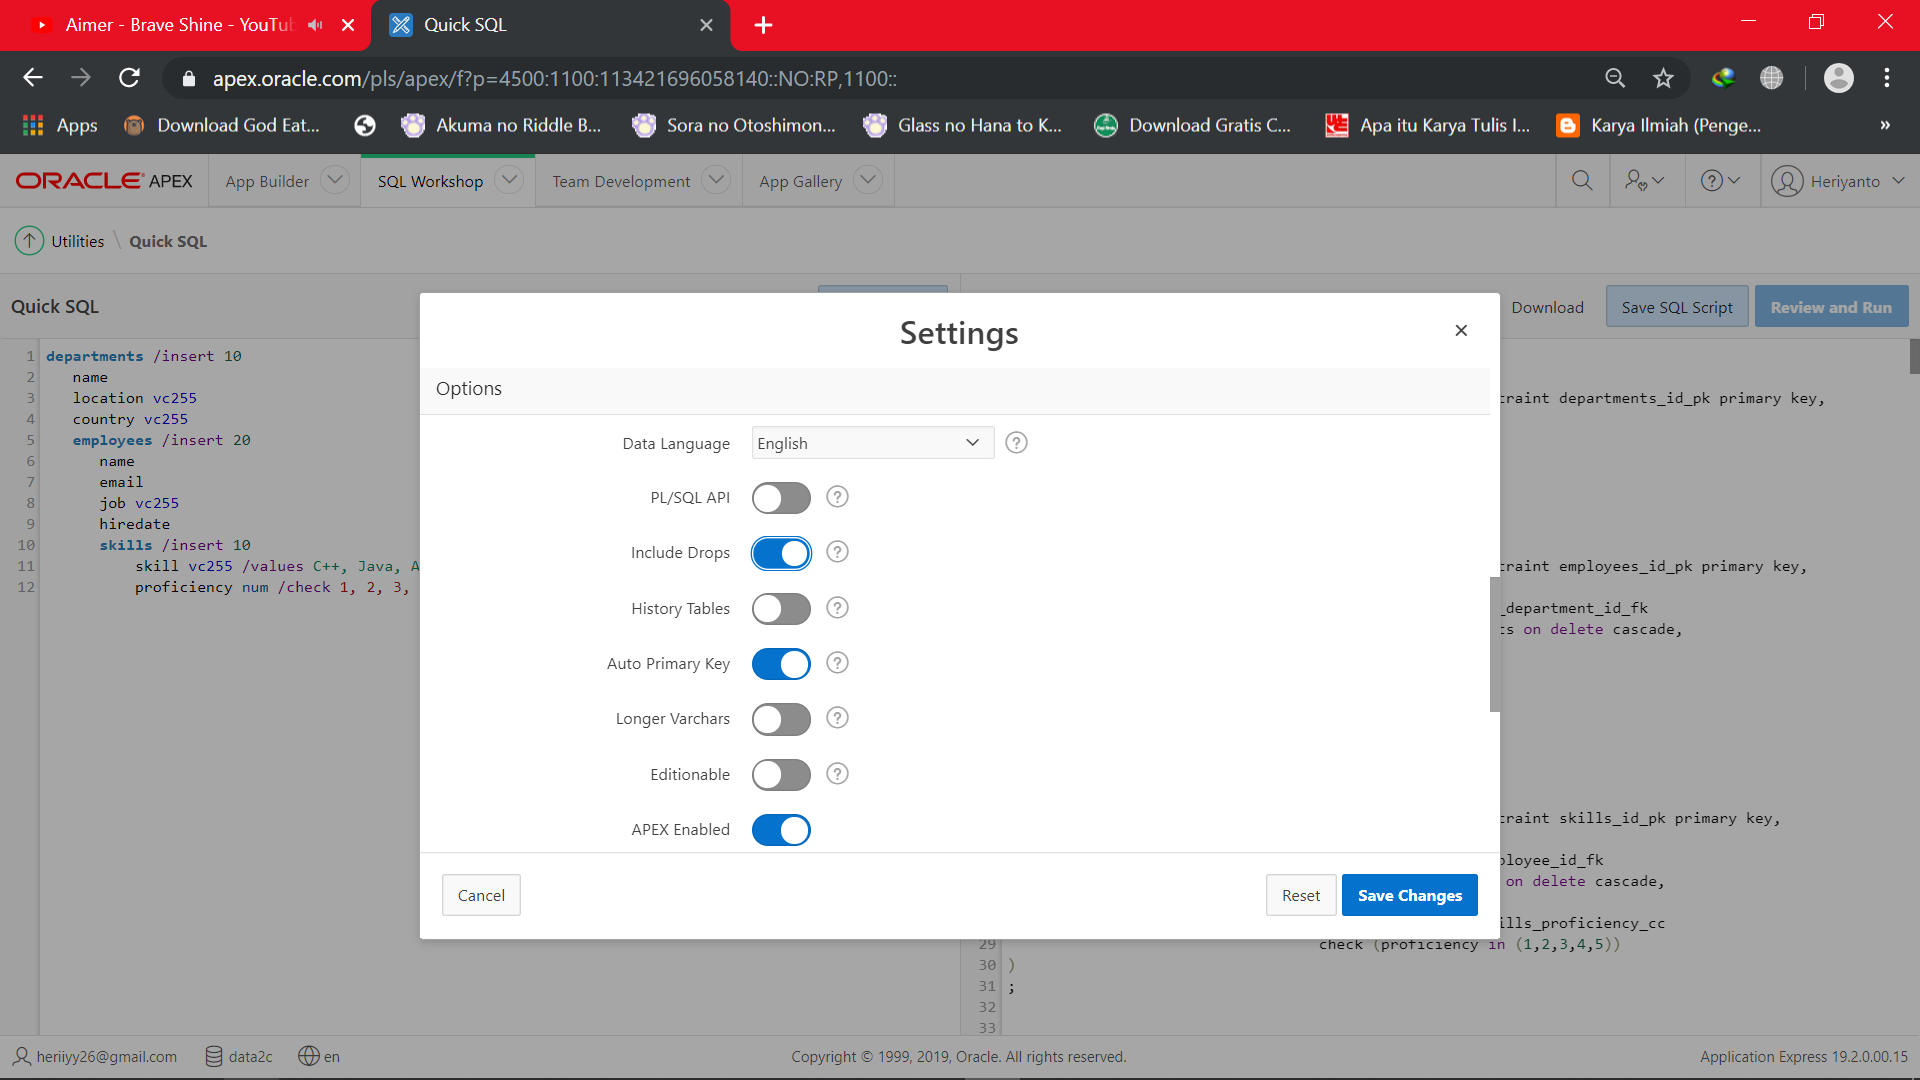
\includegraphics[width=12.5cm]{figures/Screenshot_15.png}
	\caption{Quick SQL}
\end{figure}
\item Setelah itu akan ada perubahan pada tab SQL, bisa di lihat di bawah.
\begin{figure}[!htpb]
	\centering
	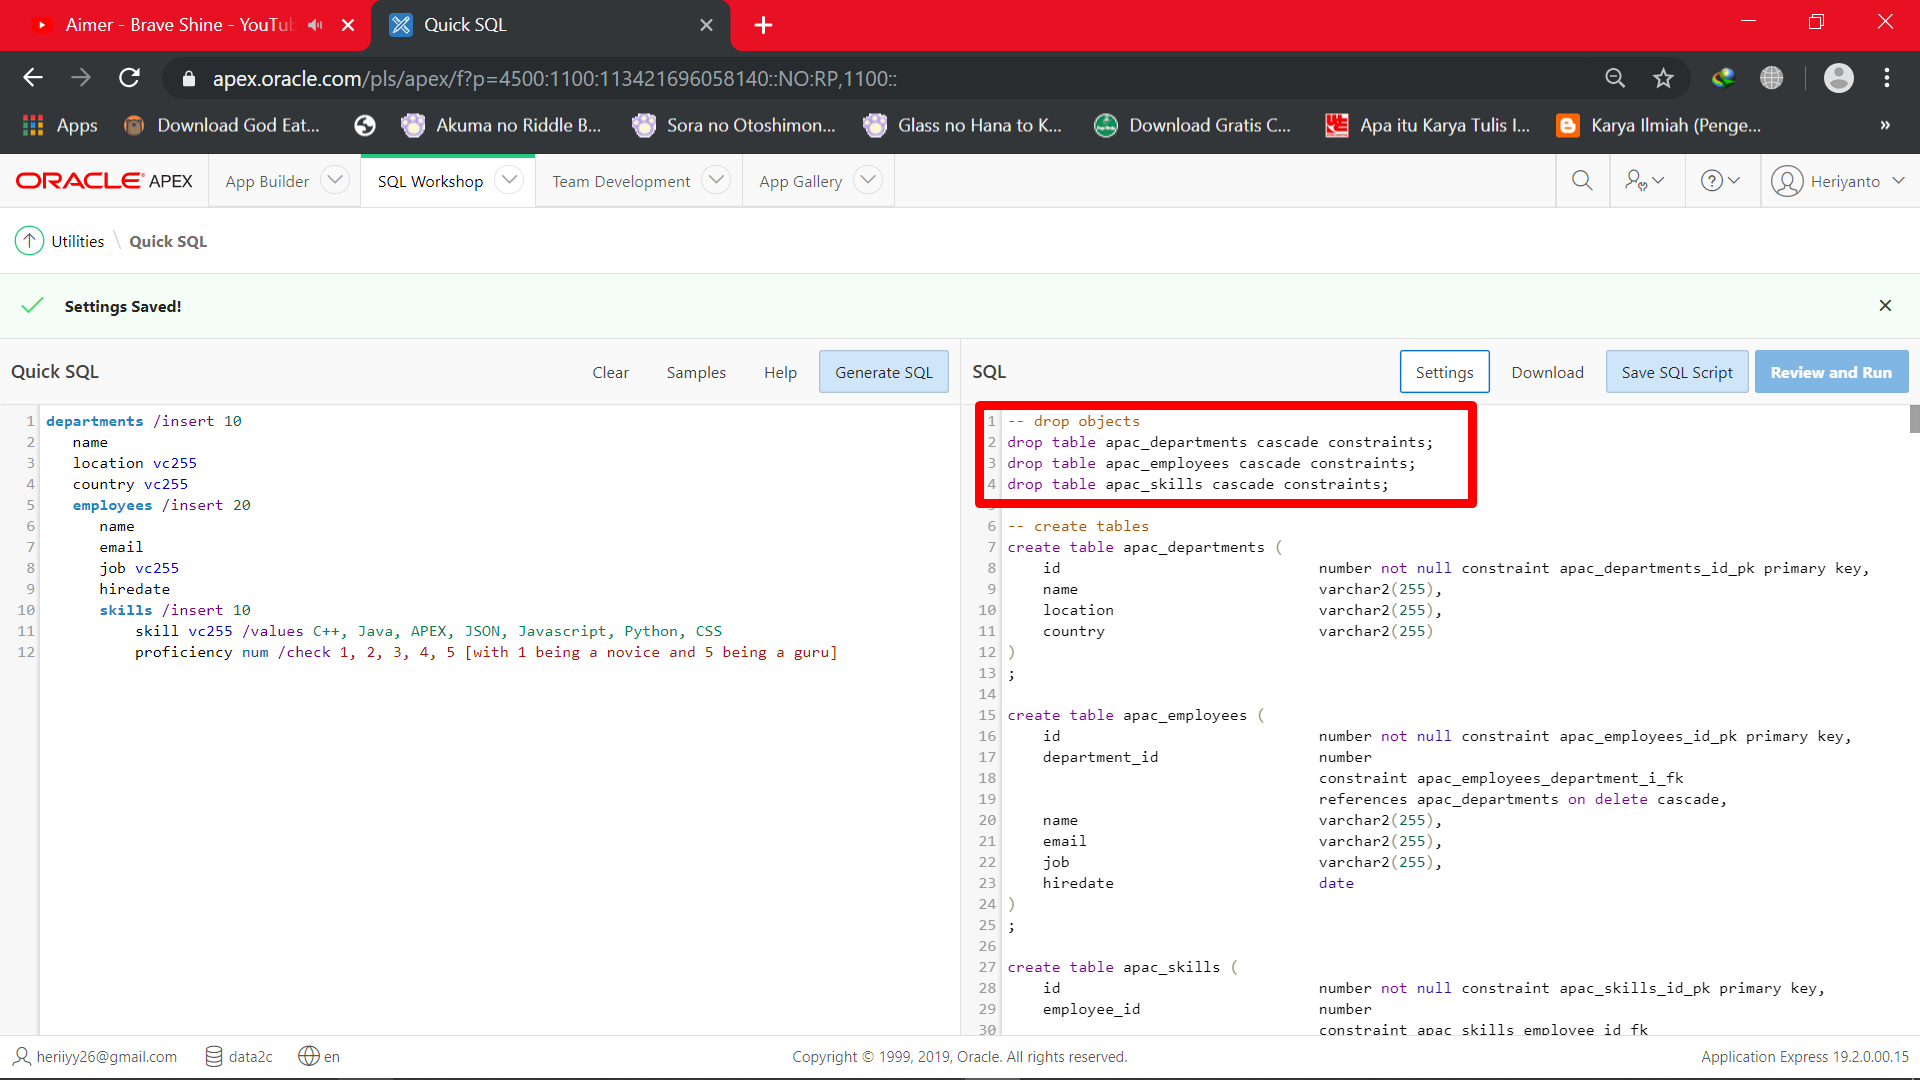
\includegraphics[width=12.5cm]{figures/Screenshot_16.png}
	\caption{Quick SQL}
\end{figure}
\item Klik "Save SQL Script" dan beri nama apac.
\begin{figure}[!htpb]
	\centering
	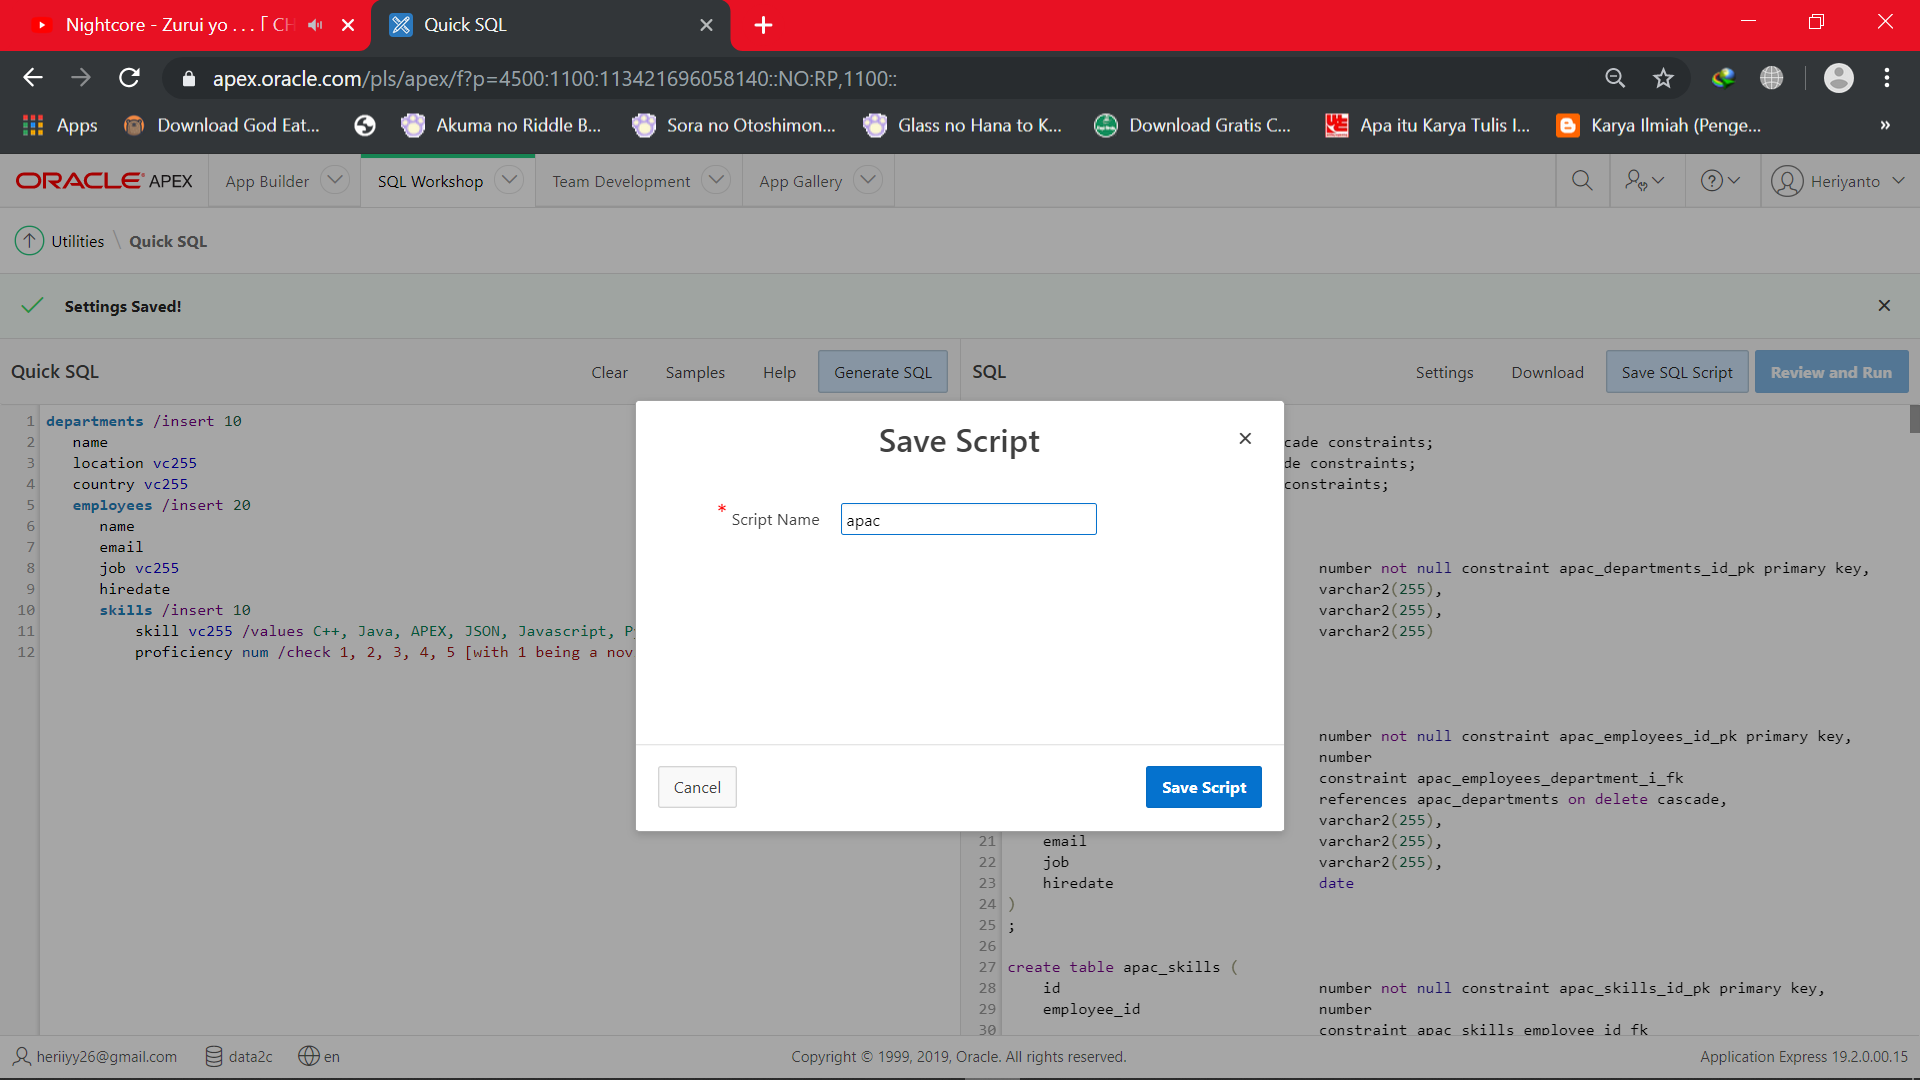
\includegraphics[width=12.5cm]{figures/Screenshot_17.png}
	\caption{Quick SQL}
\end{figure}
\item Lalu Klik "Review and Run" dan akan muncul tampilan seperti di bawah dan klik "Save".
\begin{figure}[!htpb]
	\centering
	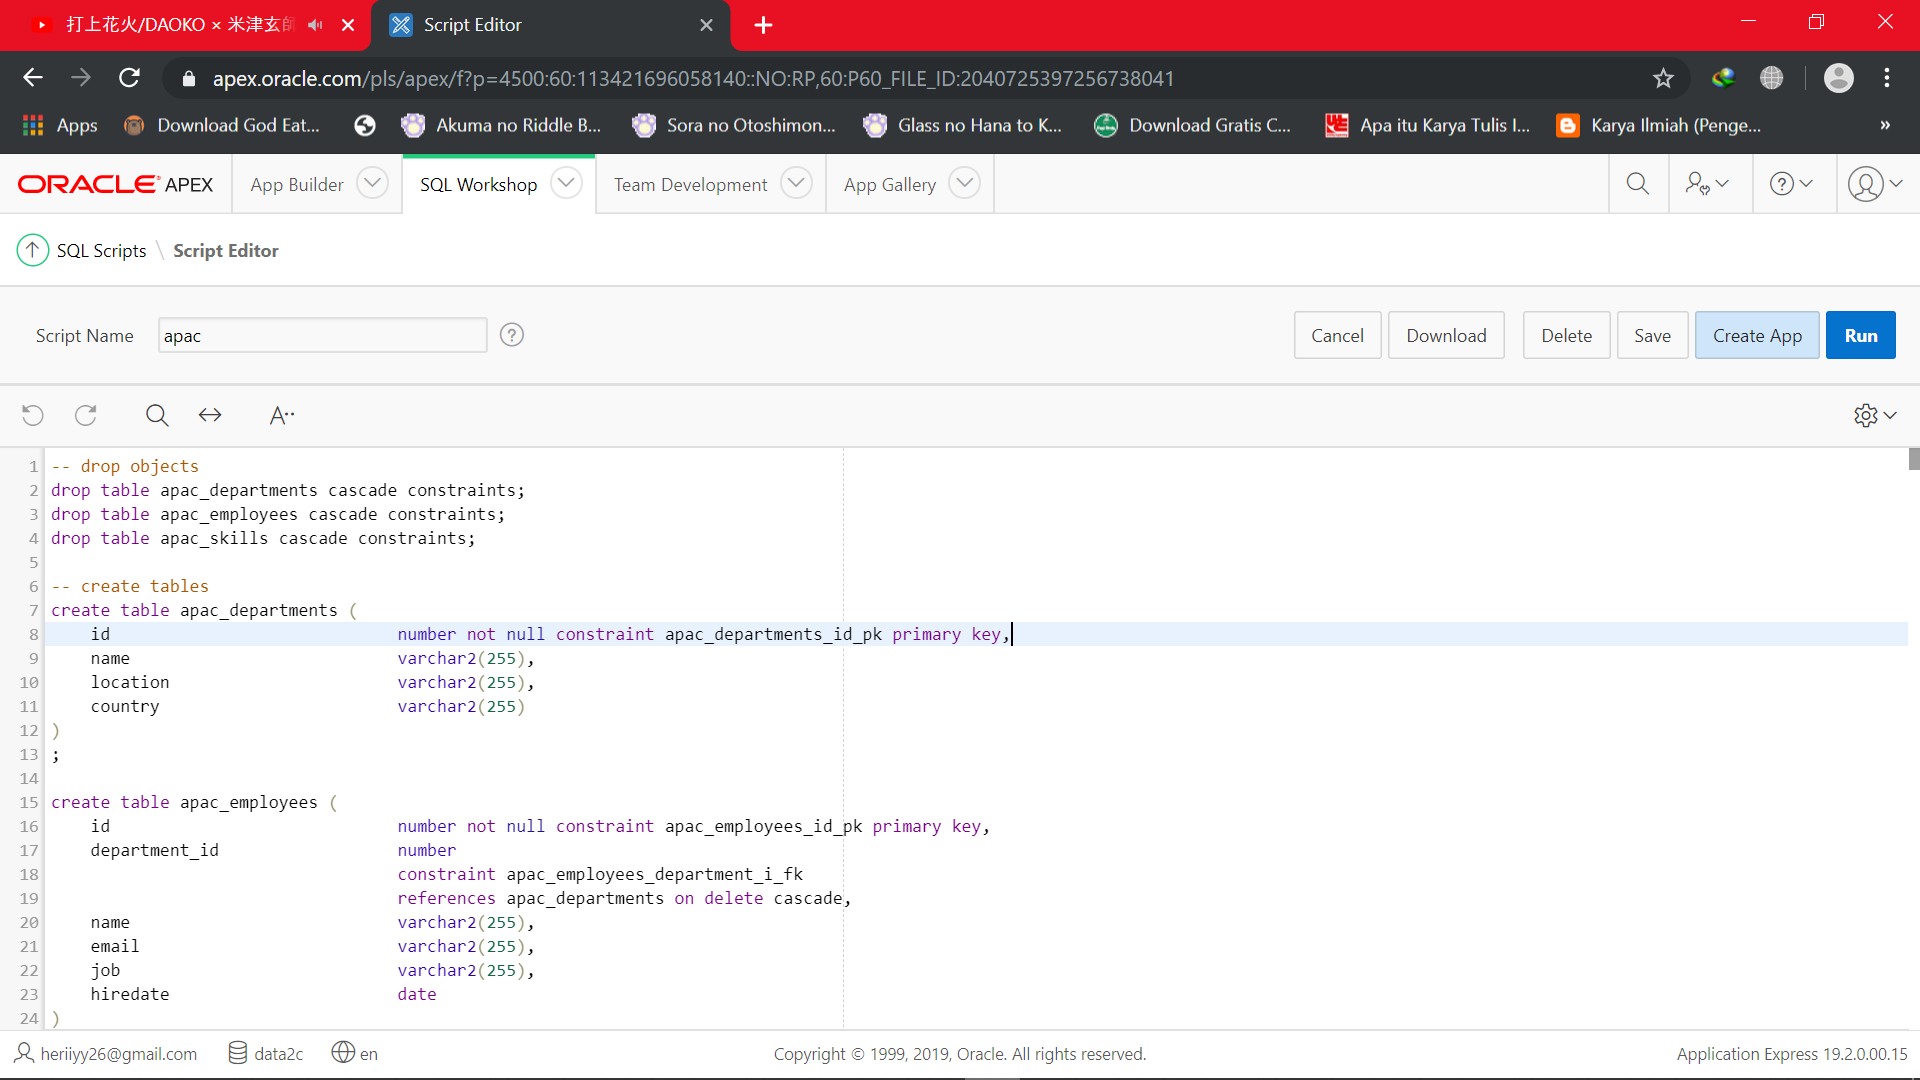
\includegraphics[width=12.5cm]{figures/Screenshot_18.png}
	\caption{Quick SQL}
\end{figure}
\item Setelah disimpan akan dialihkan ke halaman SQL Scripts dimana terdapat list-list scipts yang telah dibuat. Klik "Run" pada script apac yang dibuat tadi.
\begin{figure}[!htpb]
	\centering
	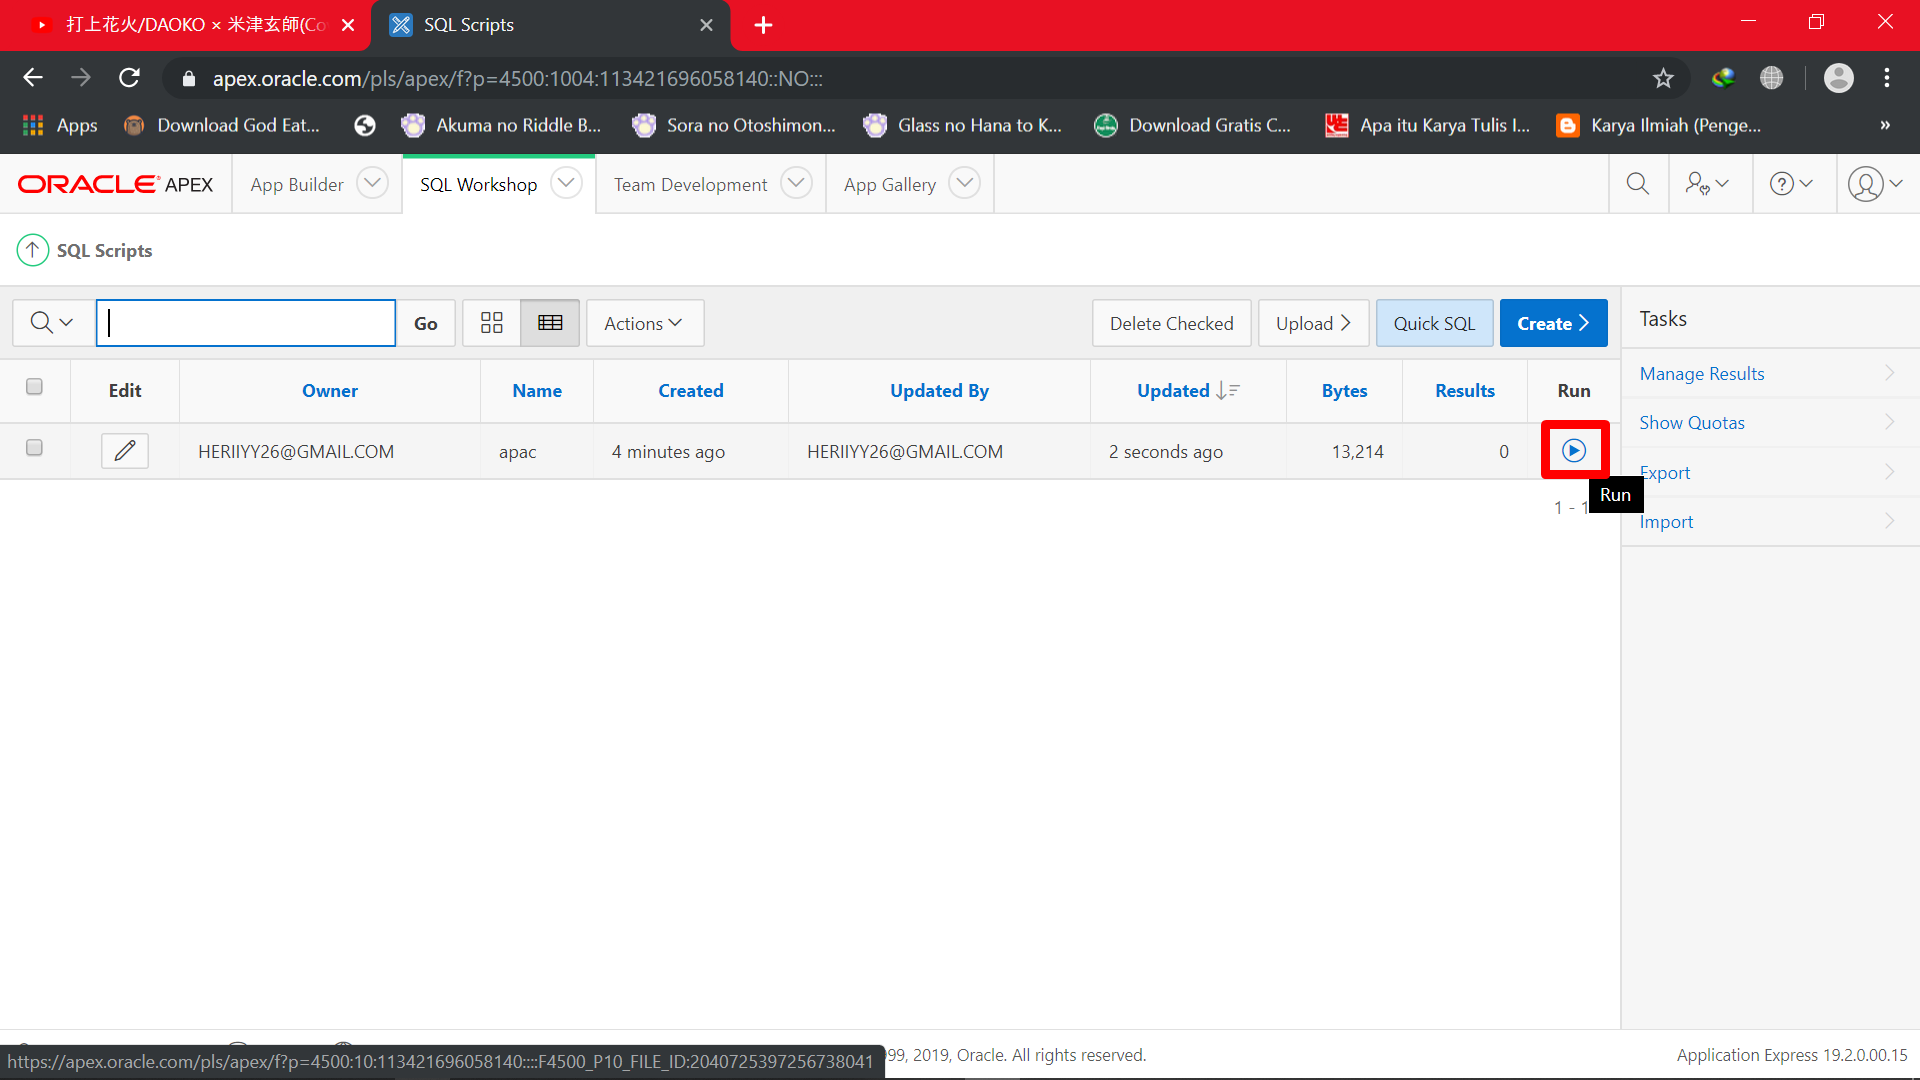
\includegraphics[width=12cm]{figures/Screenshot_19.png}
	\caption{Quick SQL}
\end{figure}
\item Lalu akan muncul halaman Run Script, Klik "Run Now".
\begin{figure}[!htpb]
	\centering
	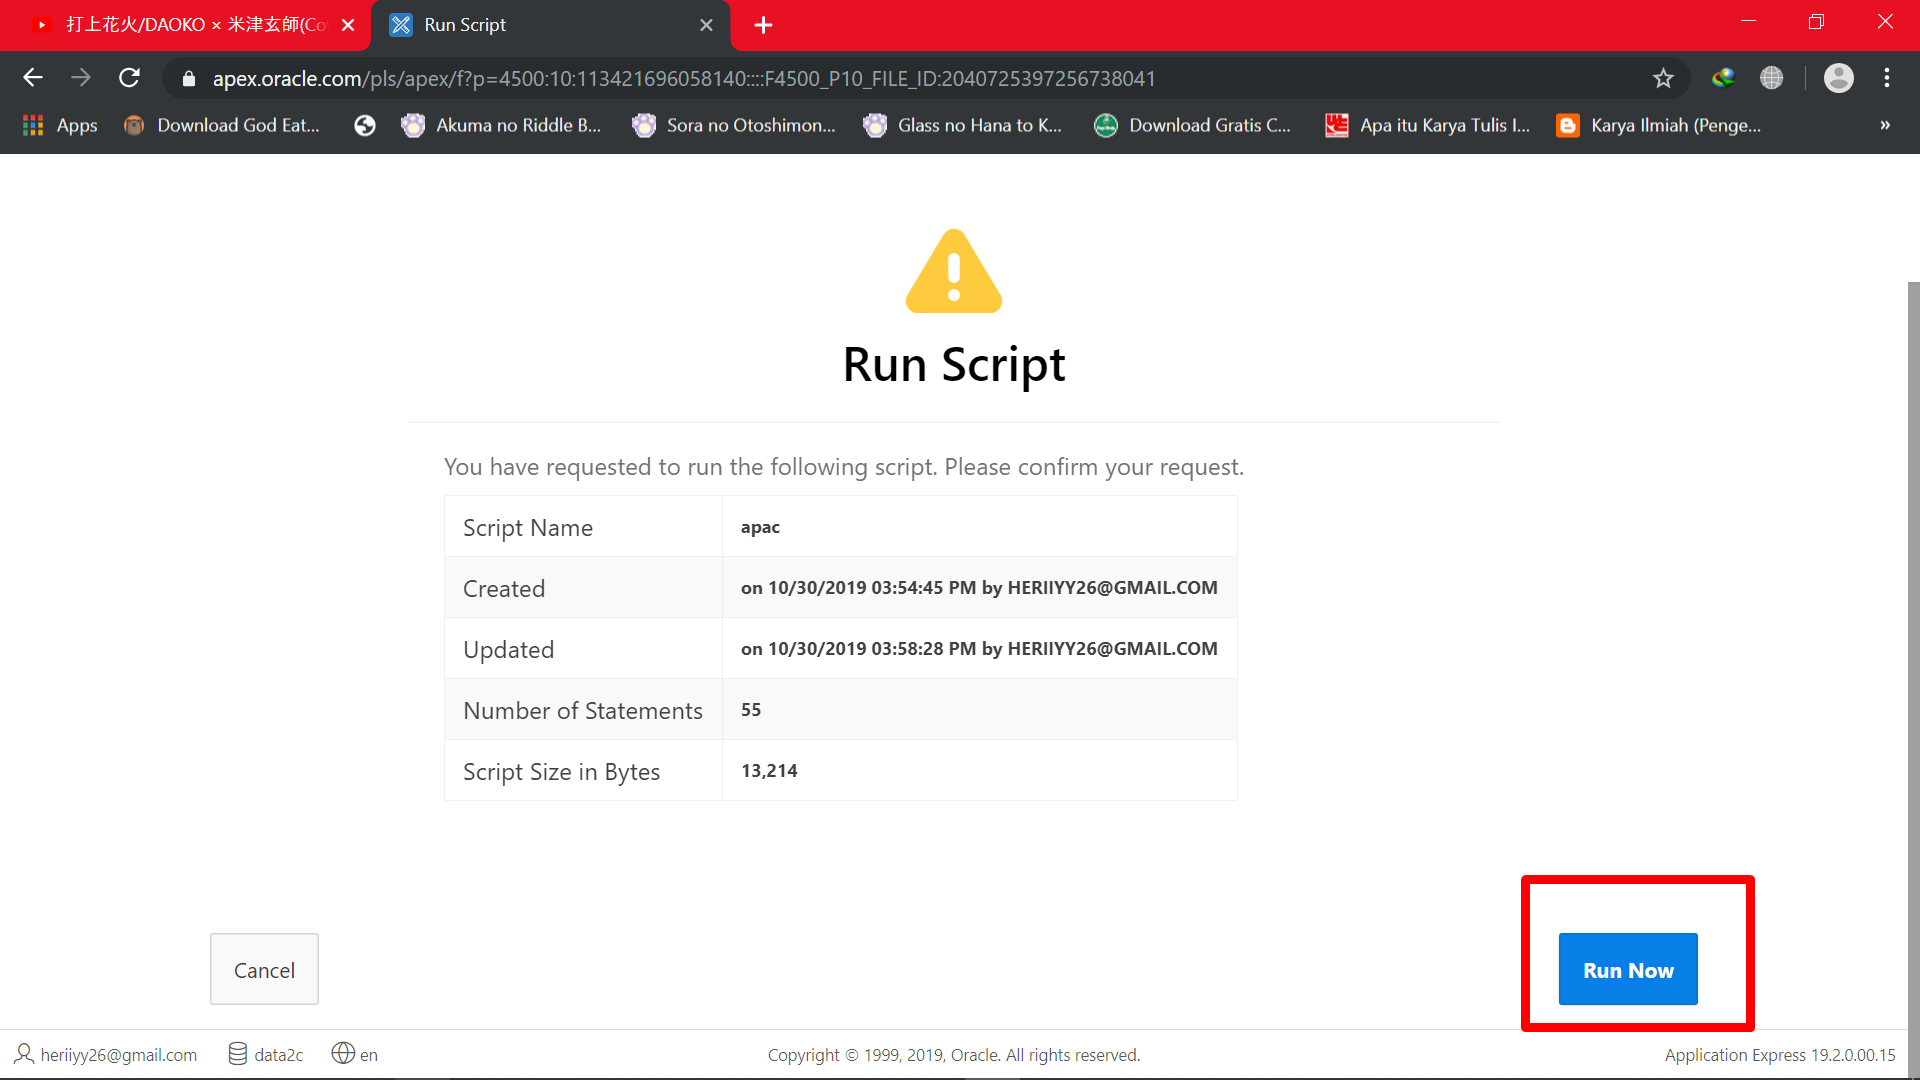
\includegraphics[width=12cm]{figures/Screenshot_20.png}
	\caption{Quick SQL}
\end{figure}
\item Akan muncul halaman Results, dimana menampilkan detail dari aplikasi yang akan dibuat.
\begin{figure}[!htpb]
	\centering
	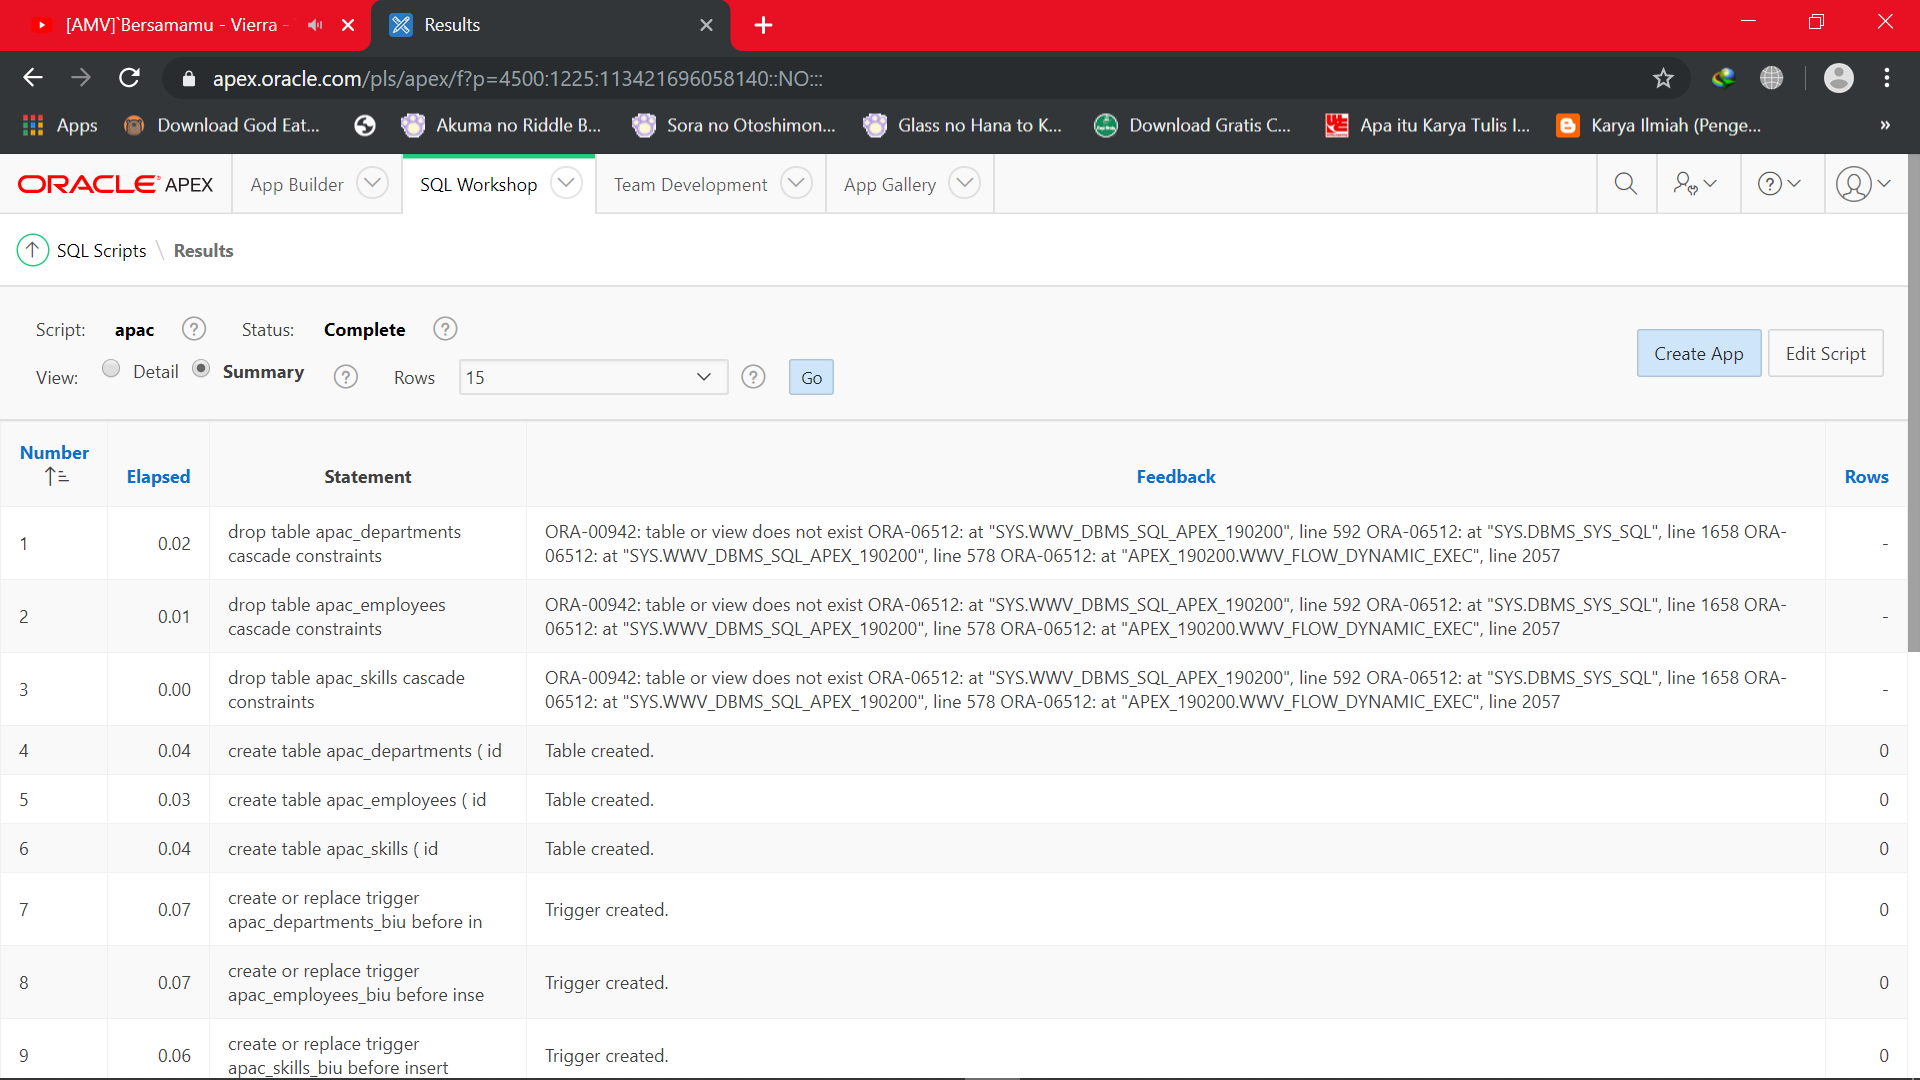
\includegraphics[width=12cm]{figures/Screenshot_21.png}
	\caption{Quick SQL}
\end{figure}
\item Lalu tekan "Create App" dan muncul kotak desicion pilih "Create Application".
\begin{figure}[!htpb]
	\centering
	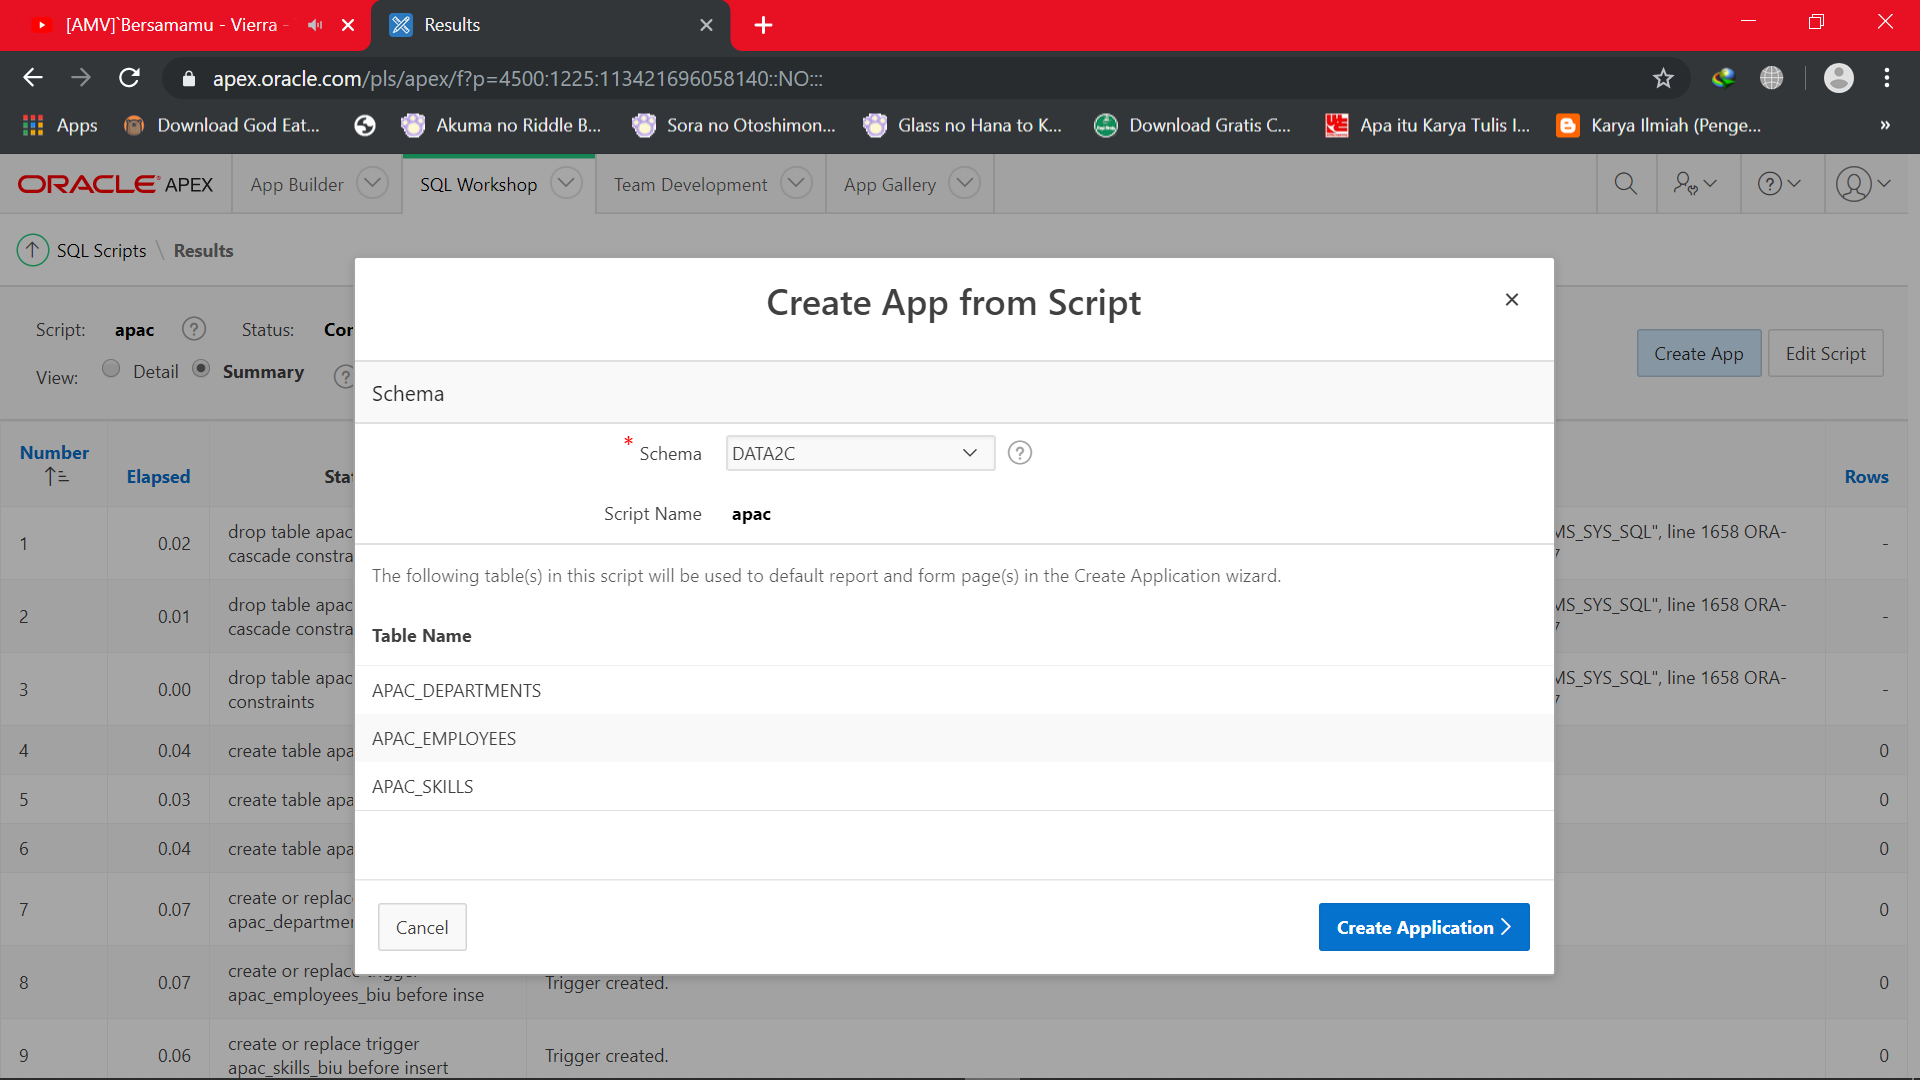
\includegraphics[width=12cm]{figures/Screenshot_22.png}
	\caption{Quick SQL}
\end{figure}
\item Jika telah dibuat silahkan Run Application lalu Login dan terakhir halaman aplikasinya akan muncul dan selesai membuat aplikasi APAC-nya.
\begin{figure}[!htpb]
	\centering
	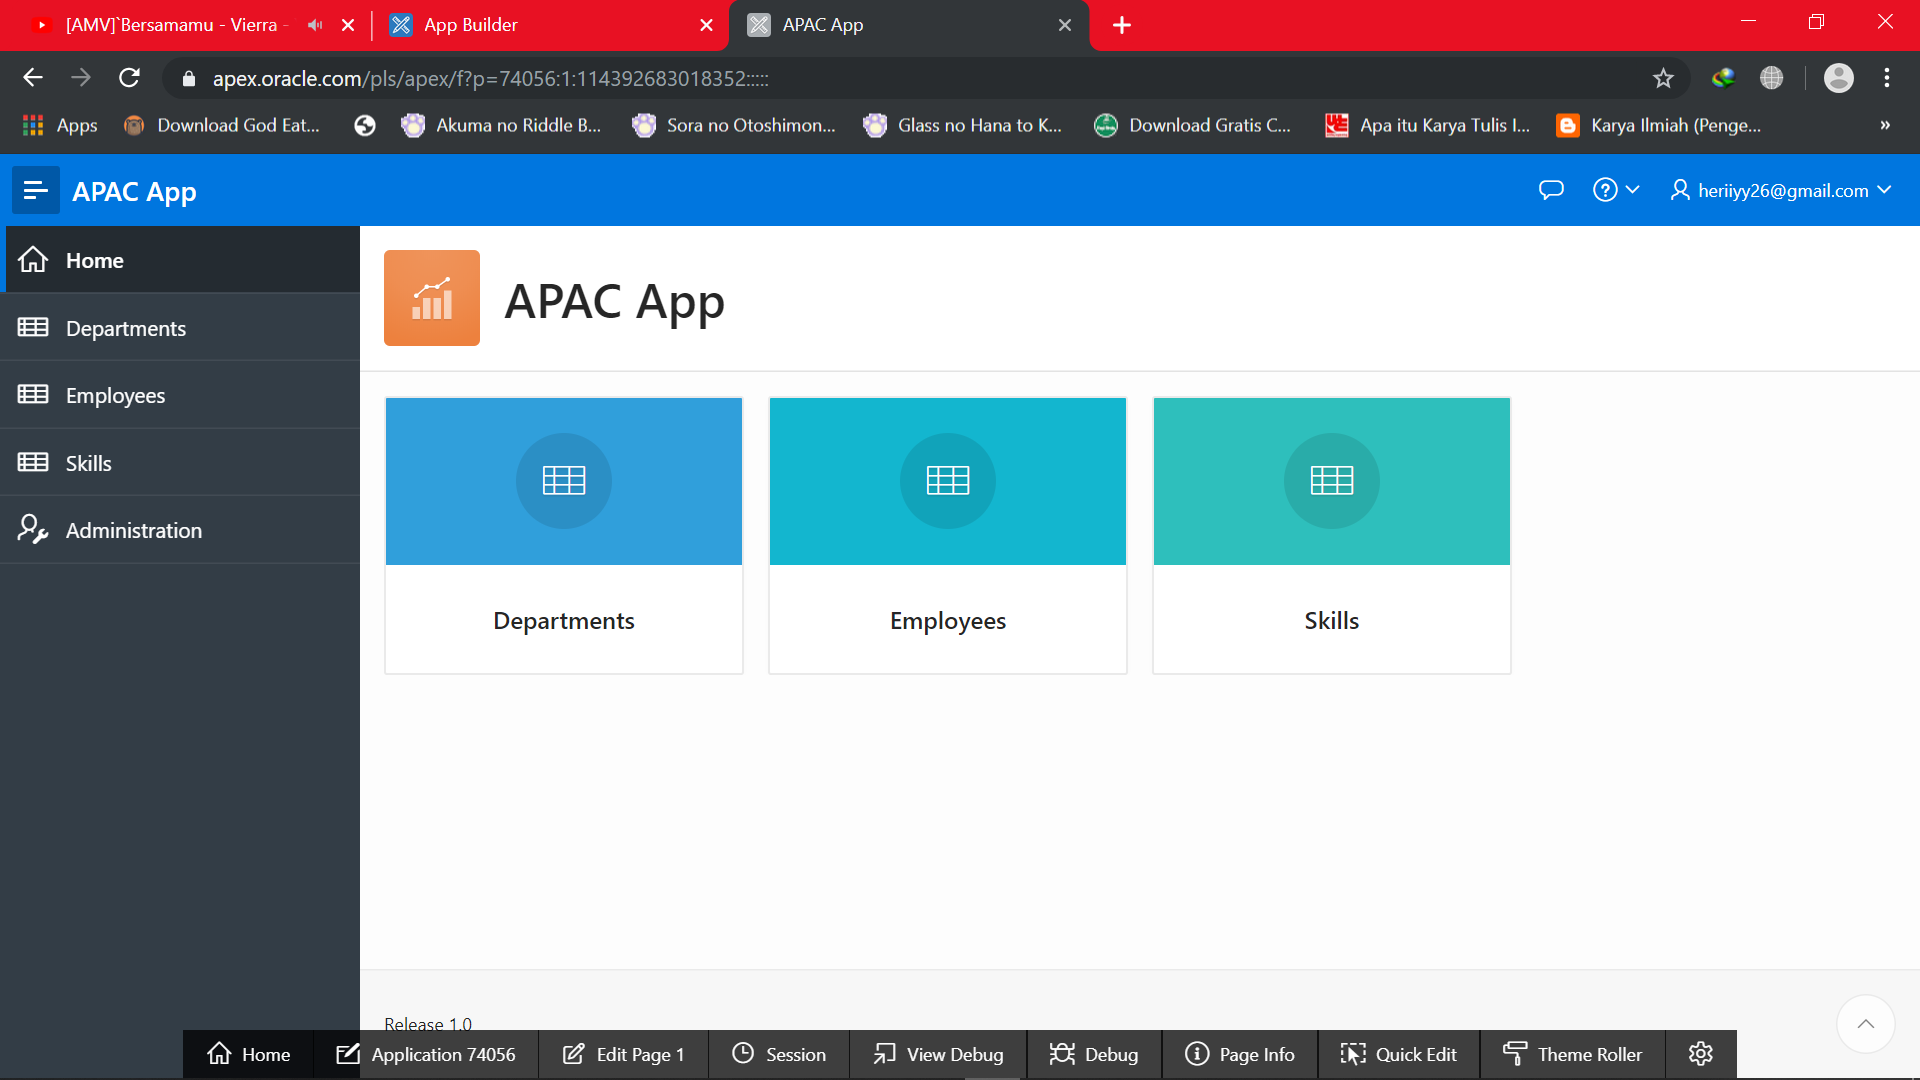
\includegraphics[width=12cm]{figures/Screenshot_23.png}
	\caption{Quick SQL}
\end{figure}
\end{itemize}
\section{Membuat Aplikasi dari App Gallery}
Pada App Gallery terdapat beberapa aplikasi yang sudah jadi dan untuk menggunakannya cukup di-install saja. Berikut cara menginstall aplikasi "Sample Charts".
\\
\\
\\
\\
\\
\\
\\
\\
\\
\\
\begin{itemize}
\item Seperti pada biasanya login ke apex.oracle, jika sudah klik "App Gallery".
\begin{figure}[!htpb]
	\centering
	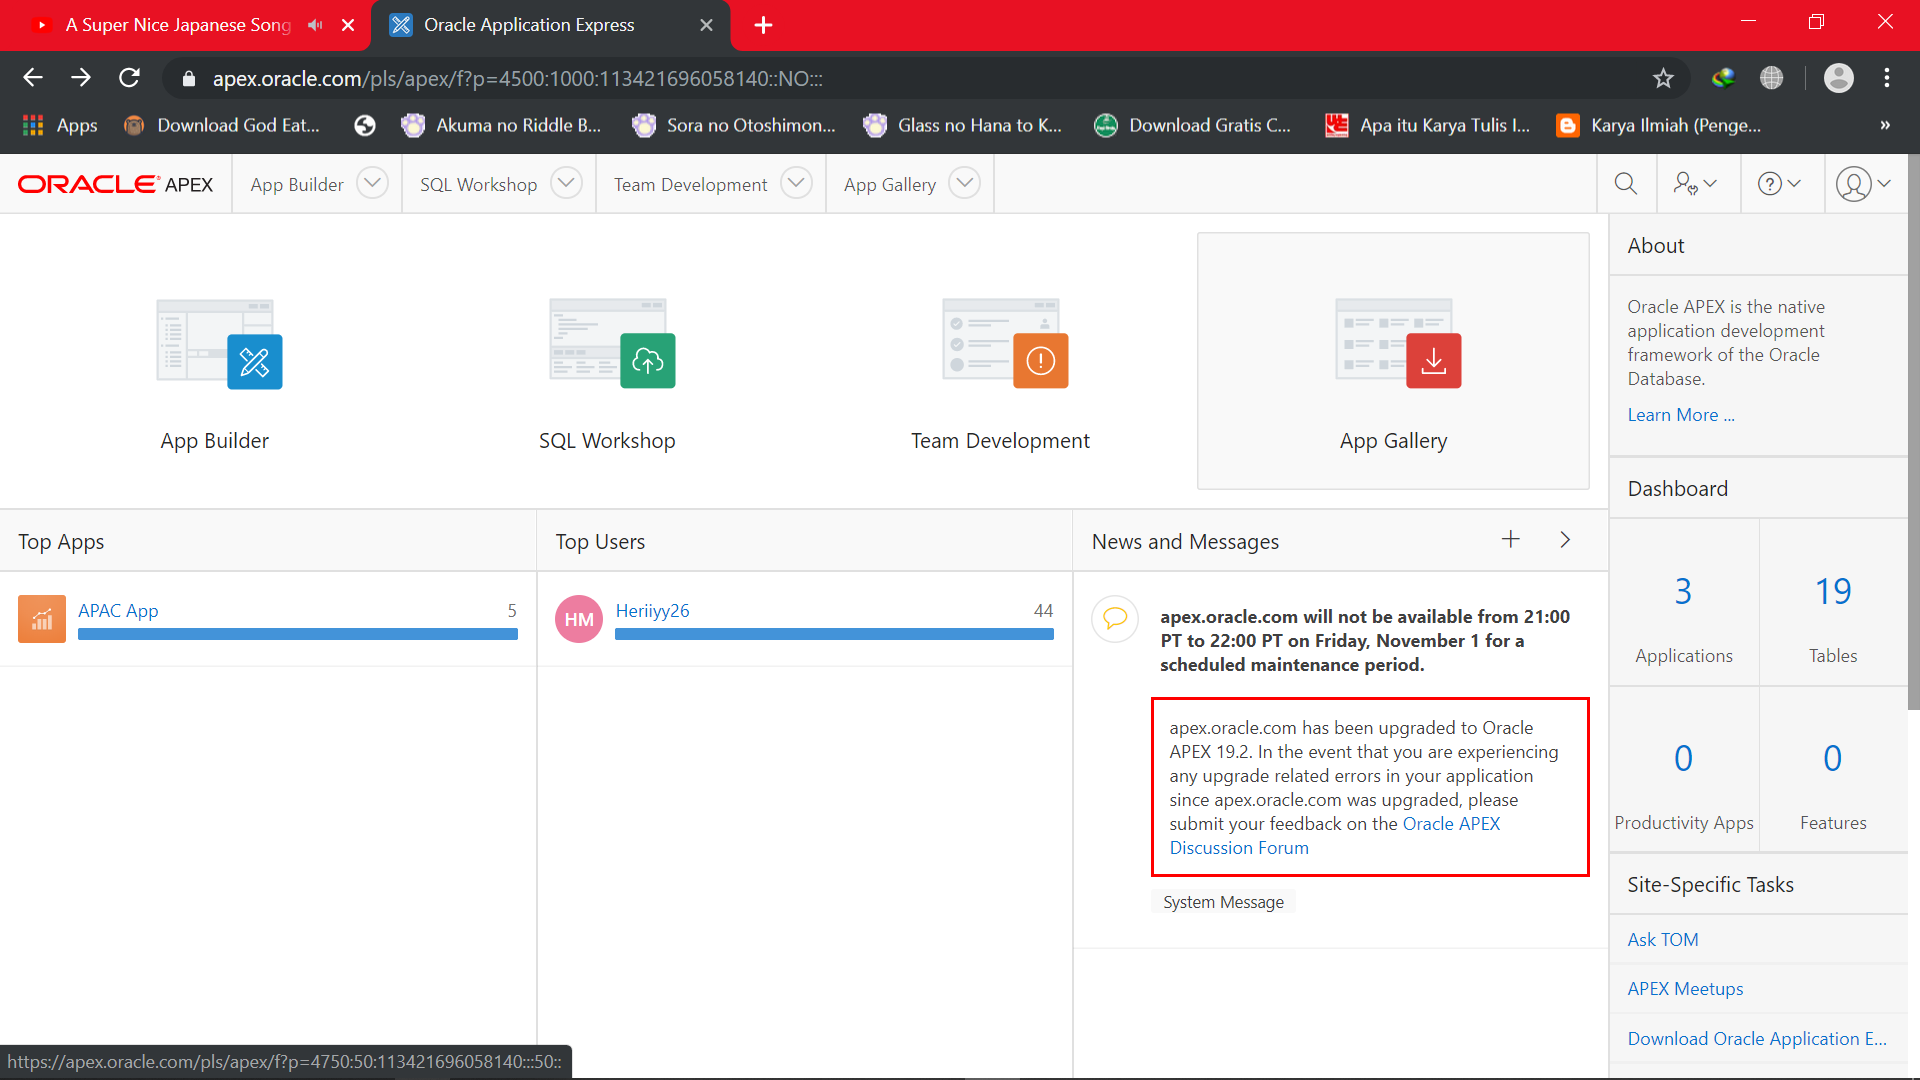
\includegraphics[width=12cm]{figures/Screenshot_24.png}
	\caption{App Gallery}
\end{figure}
\item Akan muncul halaman App Gallery dan pilih "Sample".
\begin{figure}[!htpb]
	\centering
	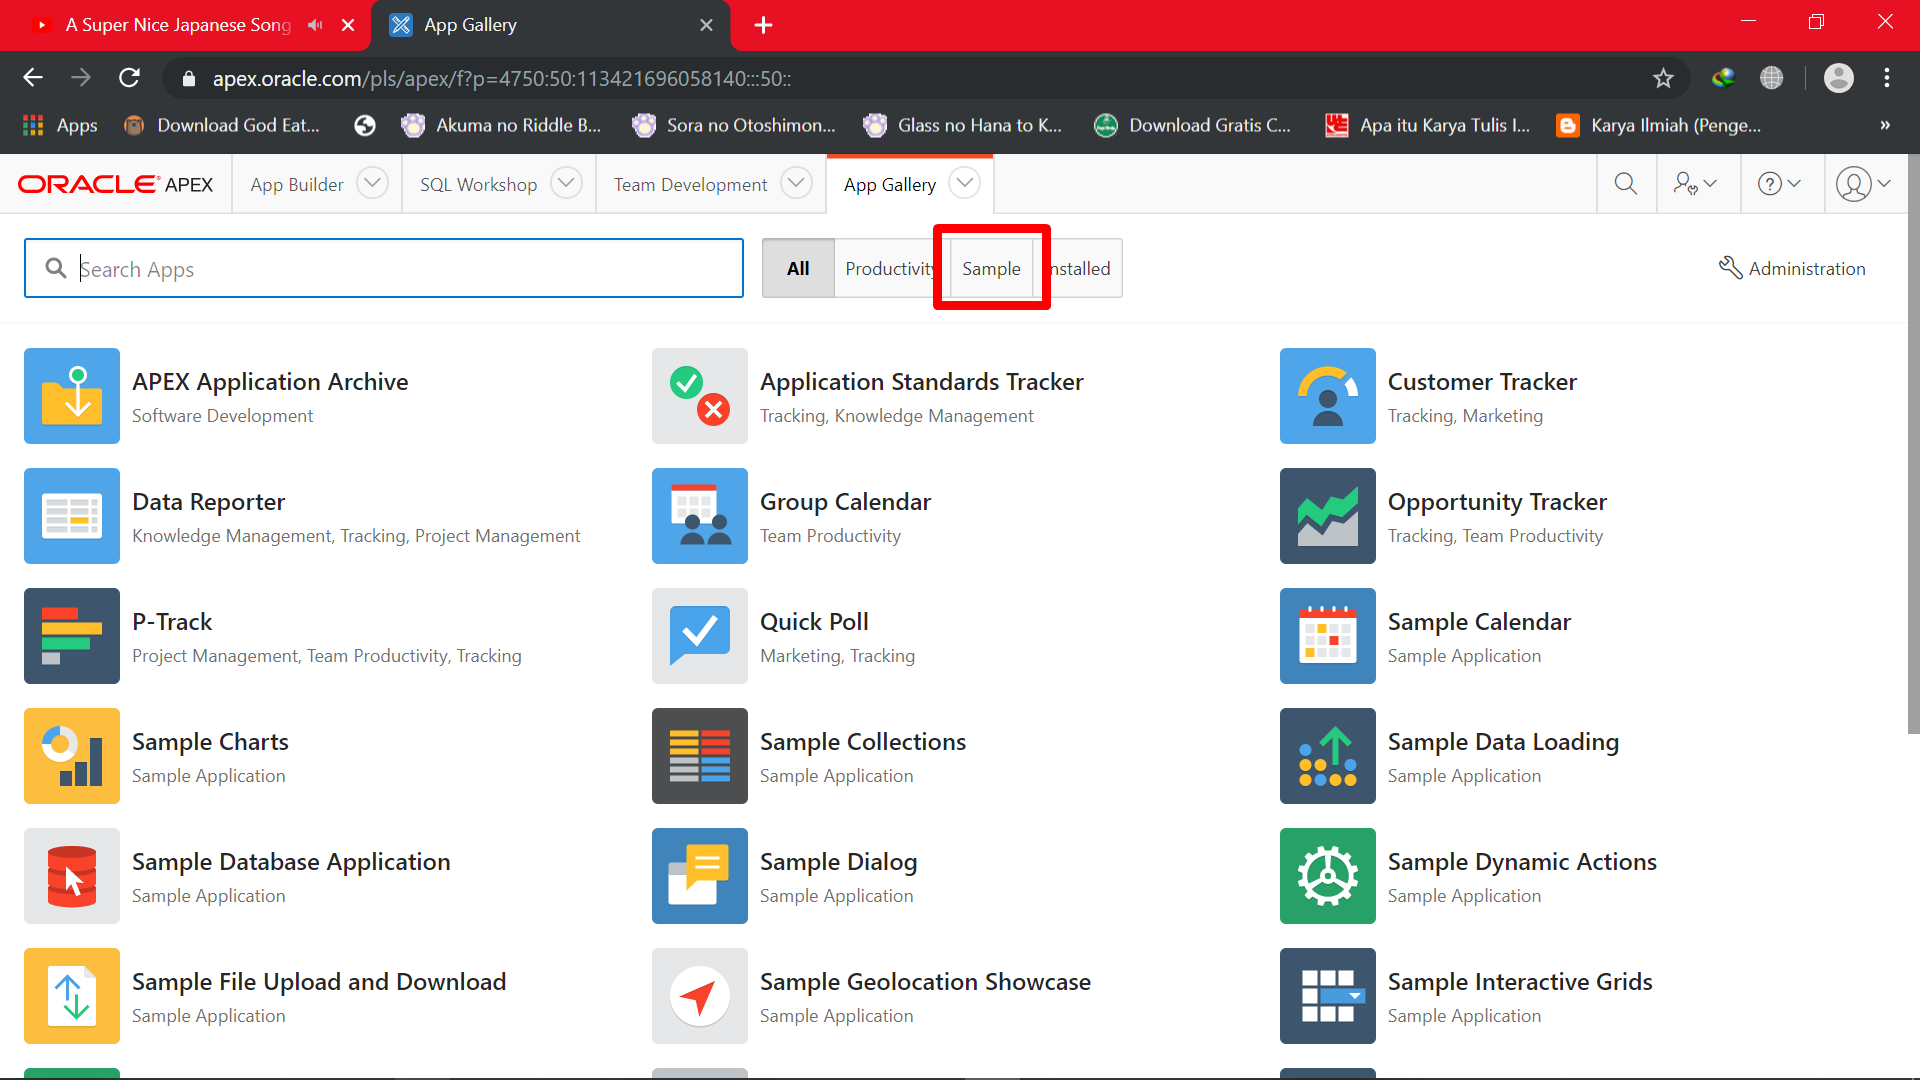
\includegraphics[width=12cm]{figures/Screenshot_25.png}
	\caption{App Gallery}
\end{figure}
\item Pilih "Sample Charts".
\begin{figure}[!htpb]
	\centering
	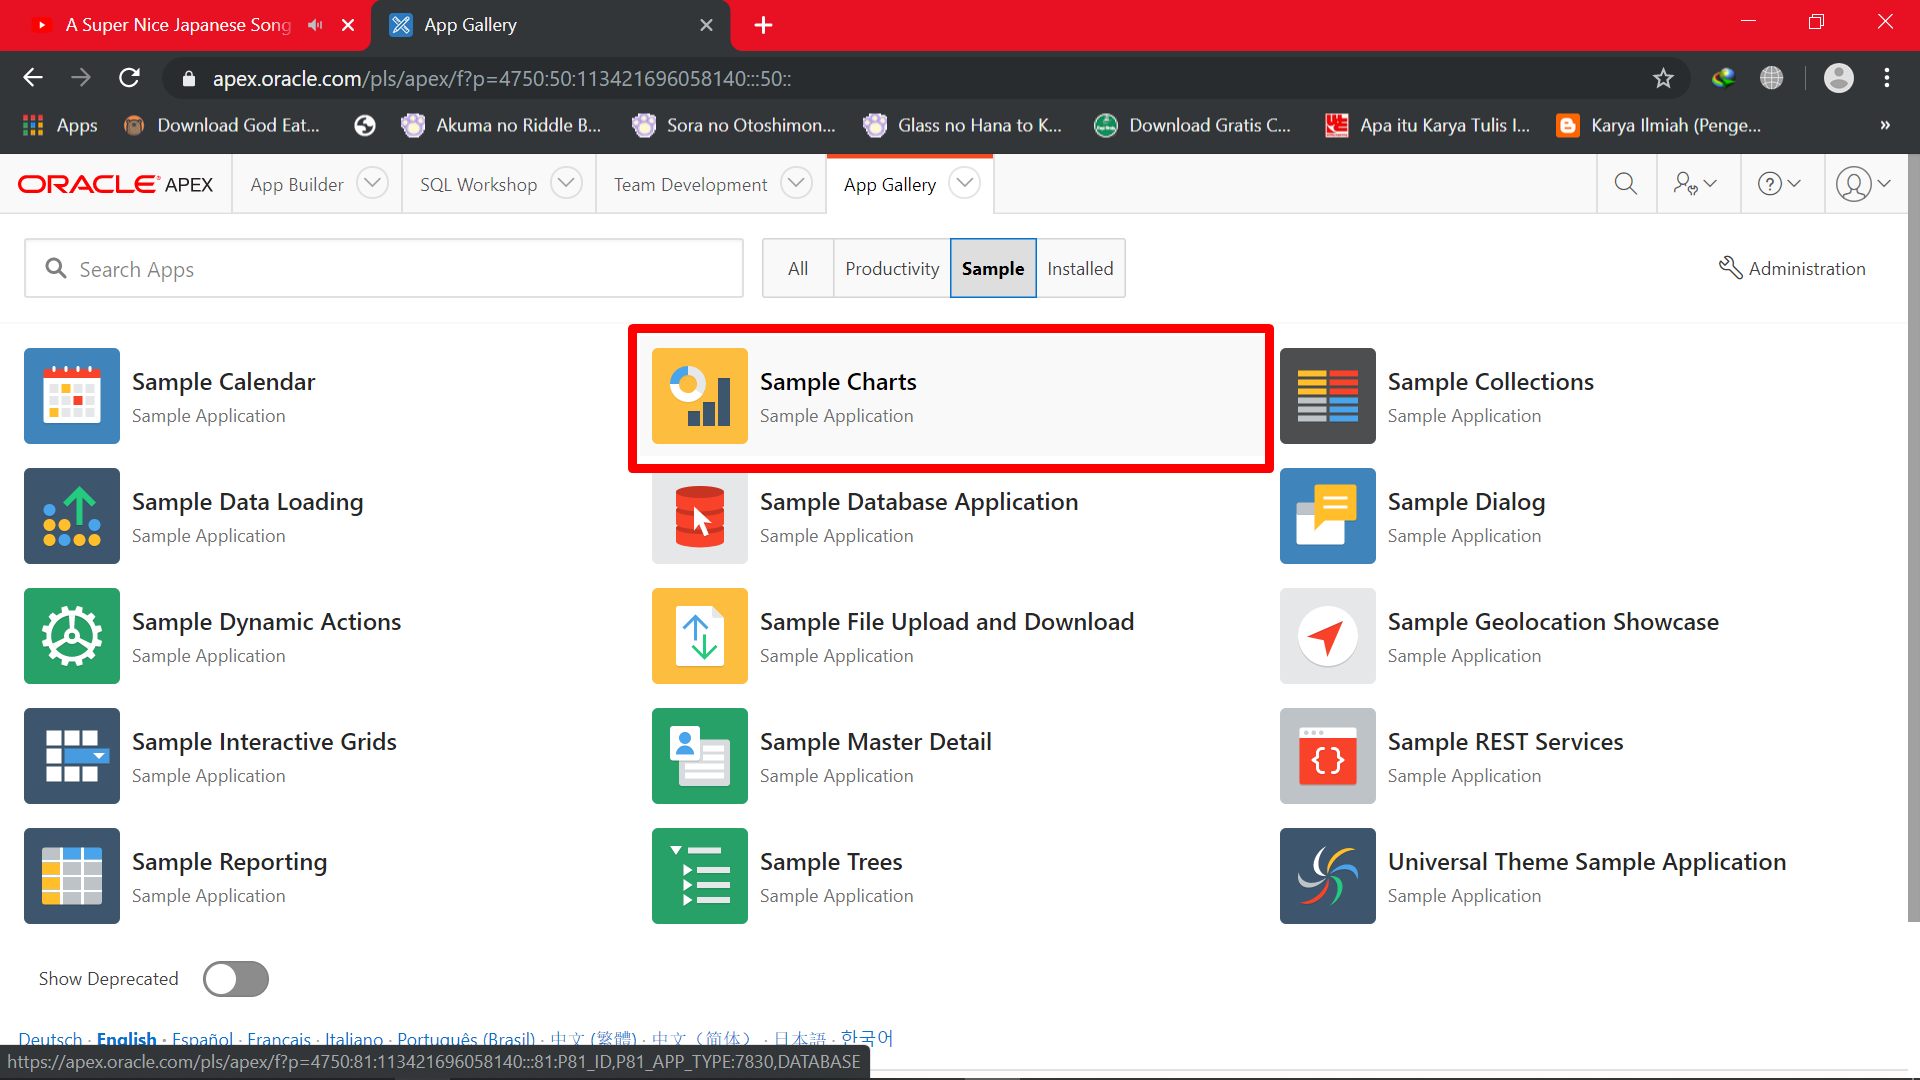
\includegraphics[width=12.5cm]{figures/Screenshot_26.png}
	\caption{App Gallery}
\end{figure}
\item Pilih "Install App".
\begin{figure}[!htpb]
	\centering
	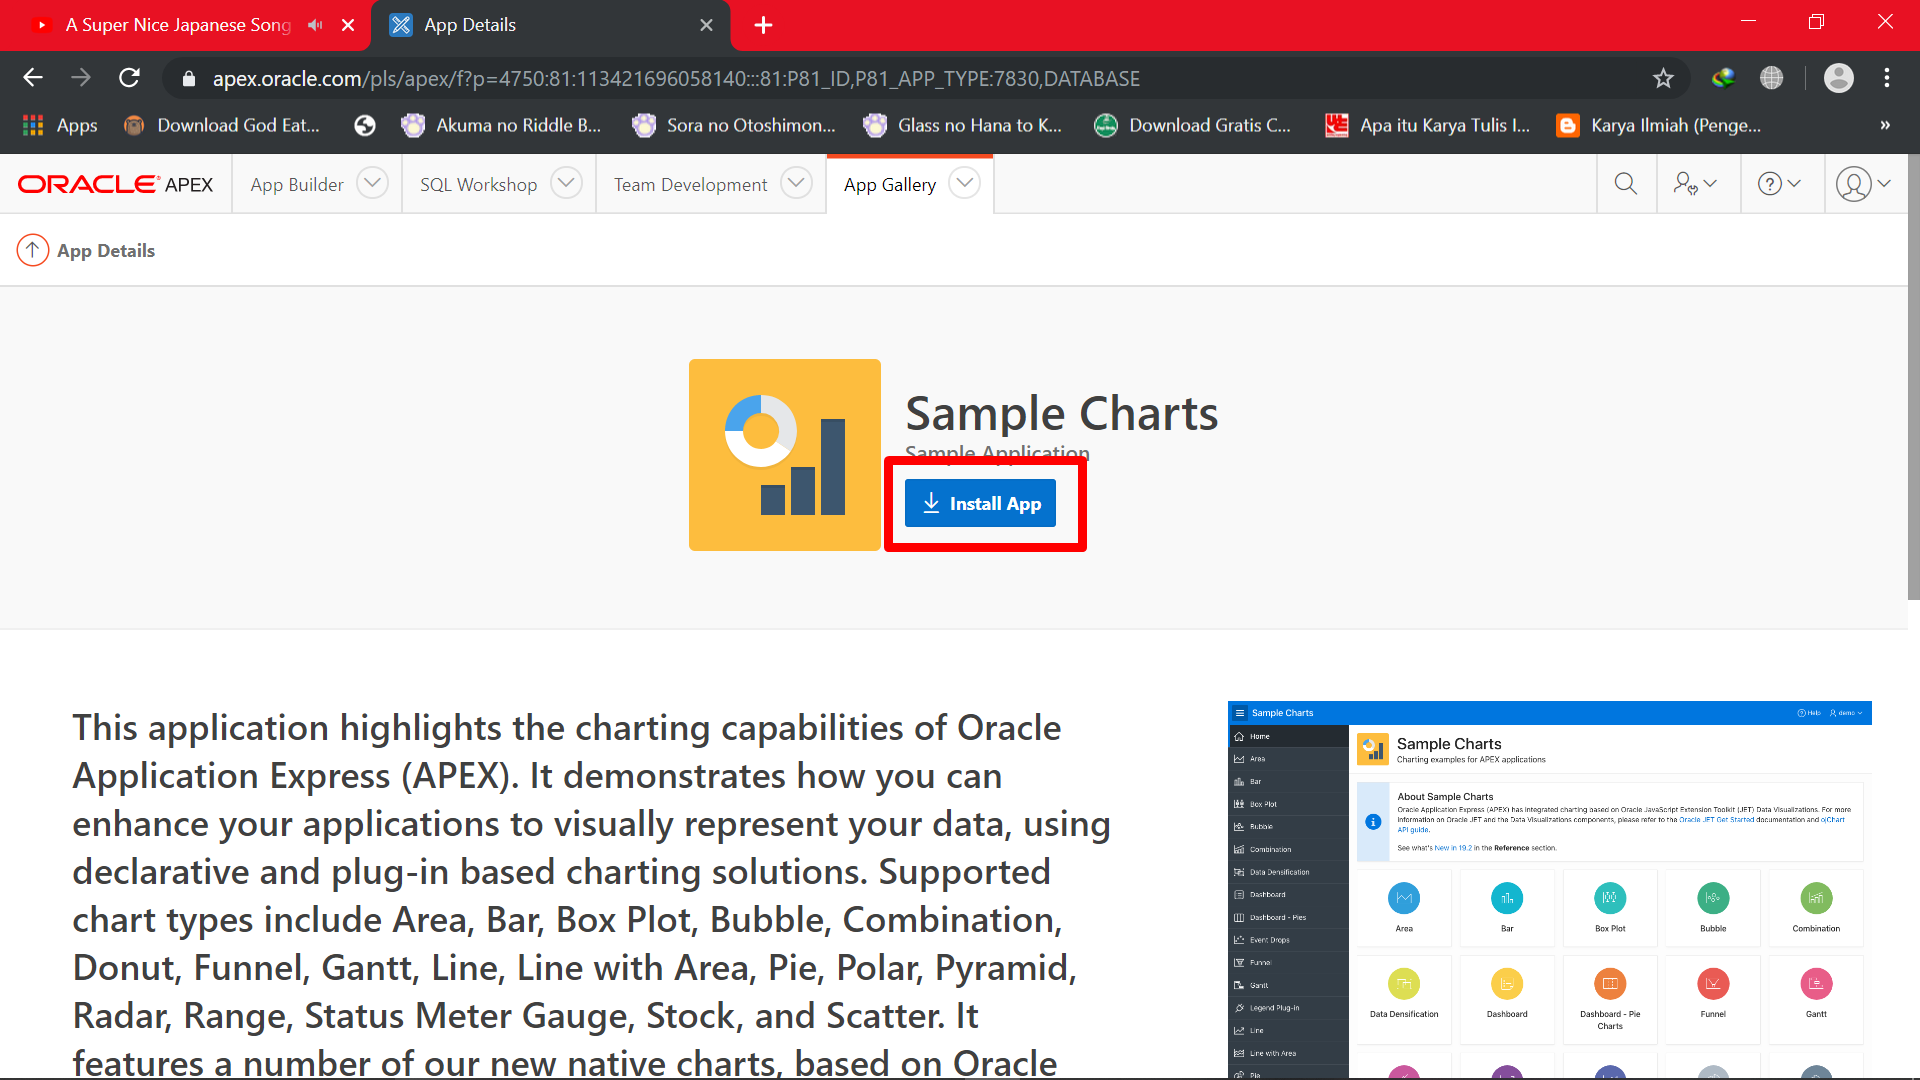
\includegraphics[width=12.5cm]{figures/Screenshot_27.png}
	\caption{App Gallery}
\end{figure}
\item Klik "Next".
\begin{figure}[!htpb]
	\centering
	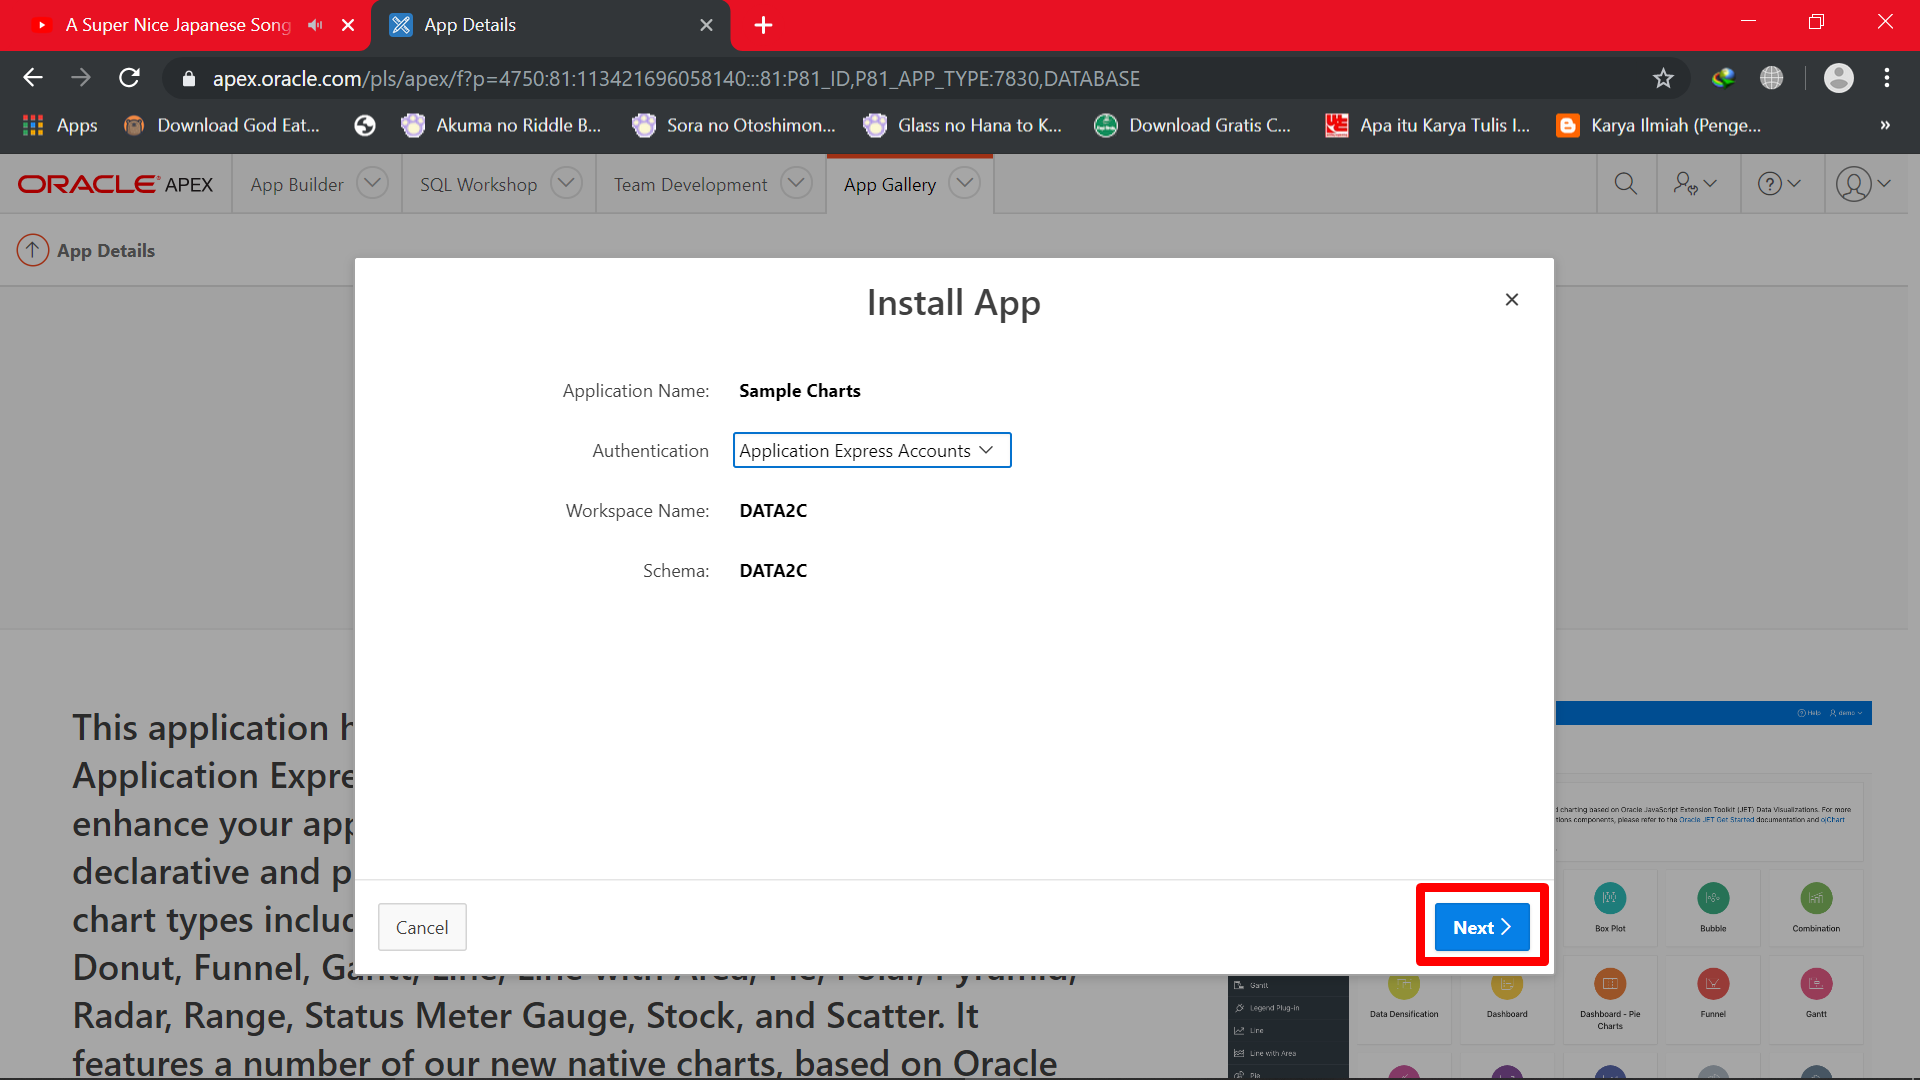
\includegraphics[width=12.5cm]{figures/Screenshot_28.png}
	\caption{App Gallery}
\end{figure}
\item Klik "Install App".
\begin{figure}[!htpb]
	\centering
	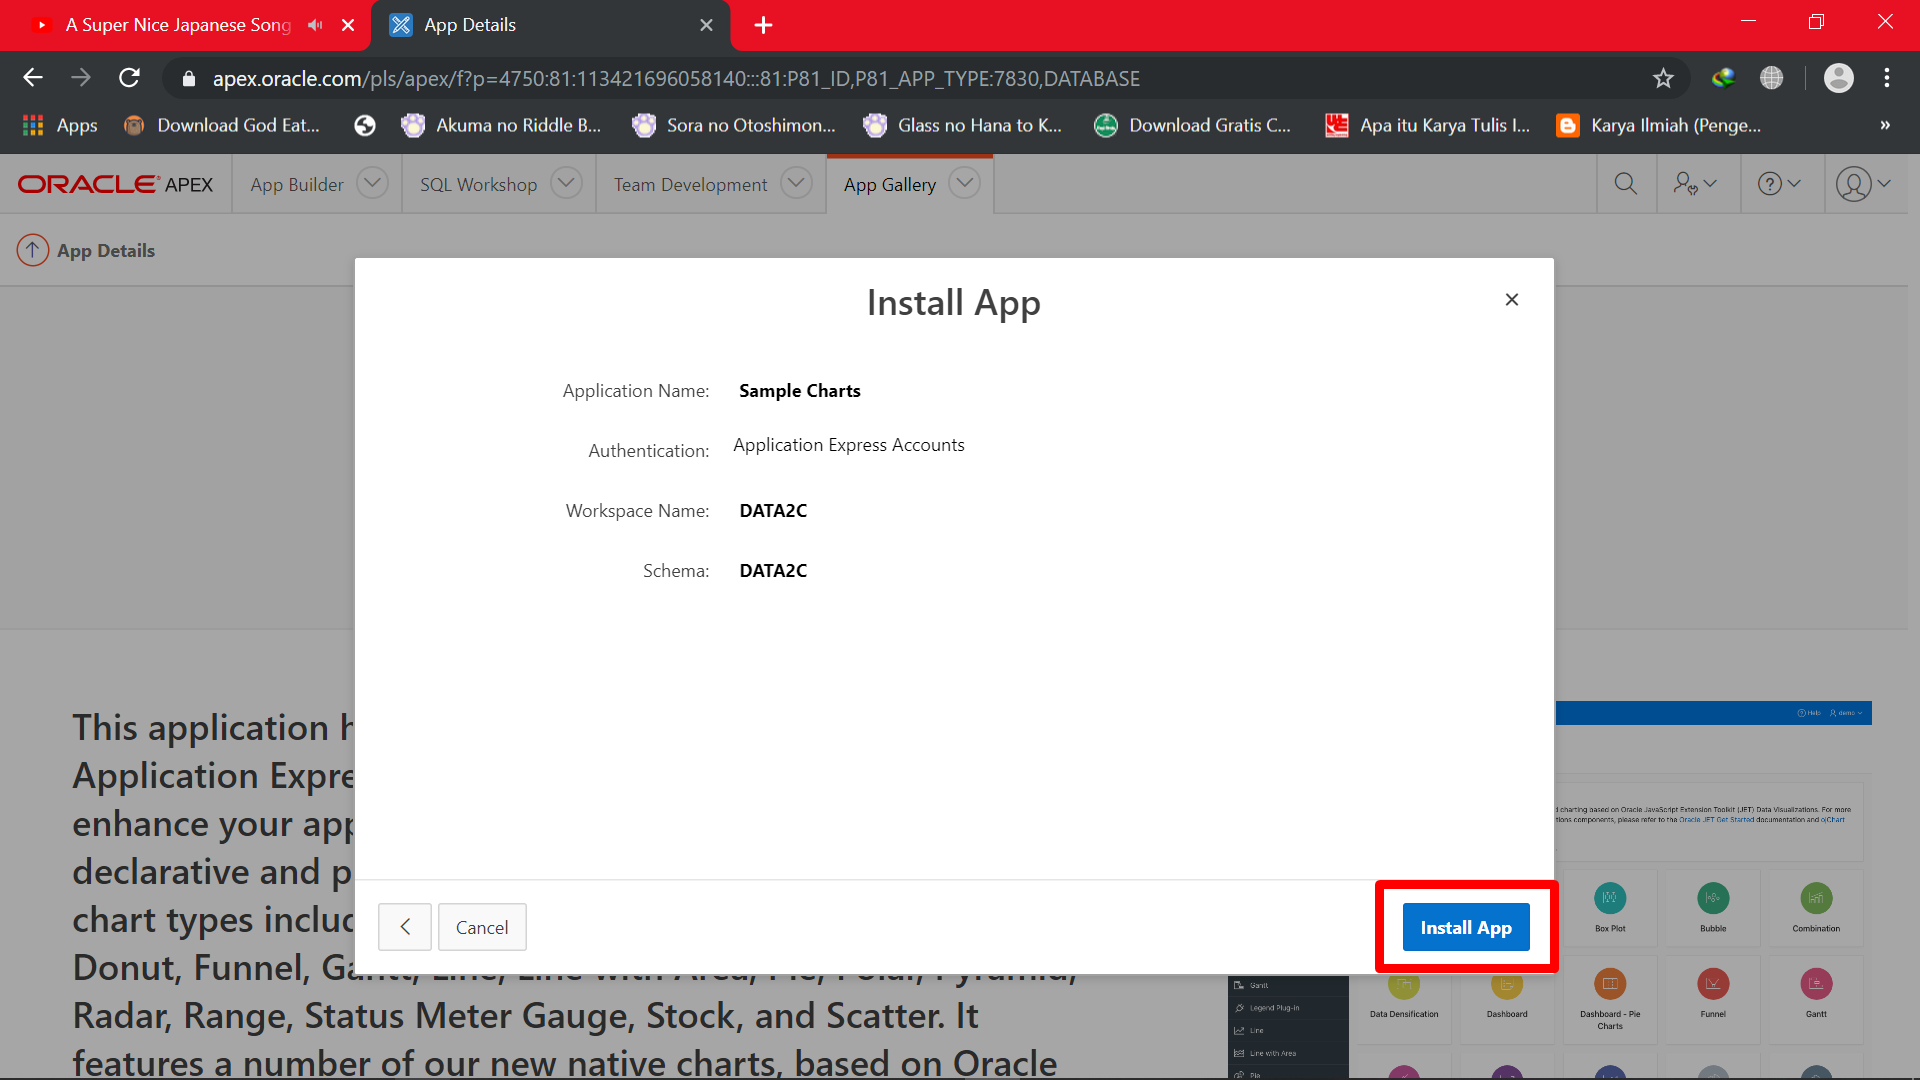
\includegraphics[width=12.5cm]{figures/Screenshot_29.png}
	\caption{App Gallery}
\end{figure}
\item Klik tombol "Run Application".
\begin{figure}[!htpb]
	\centering
	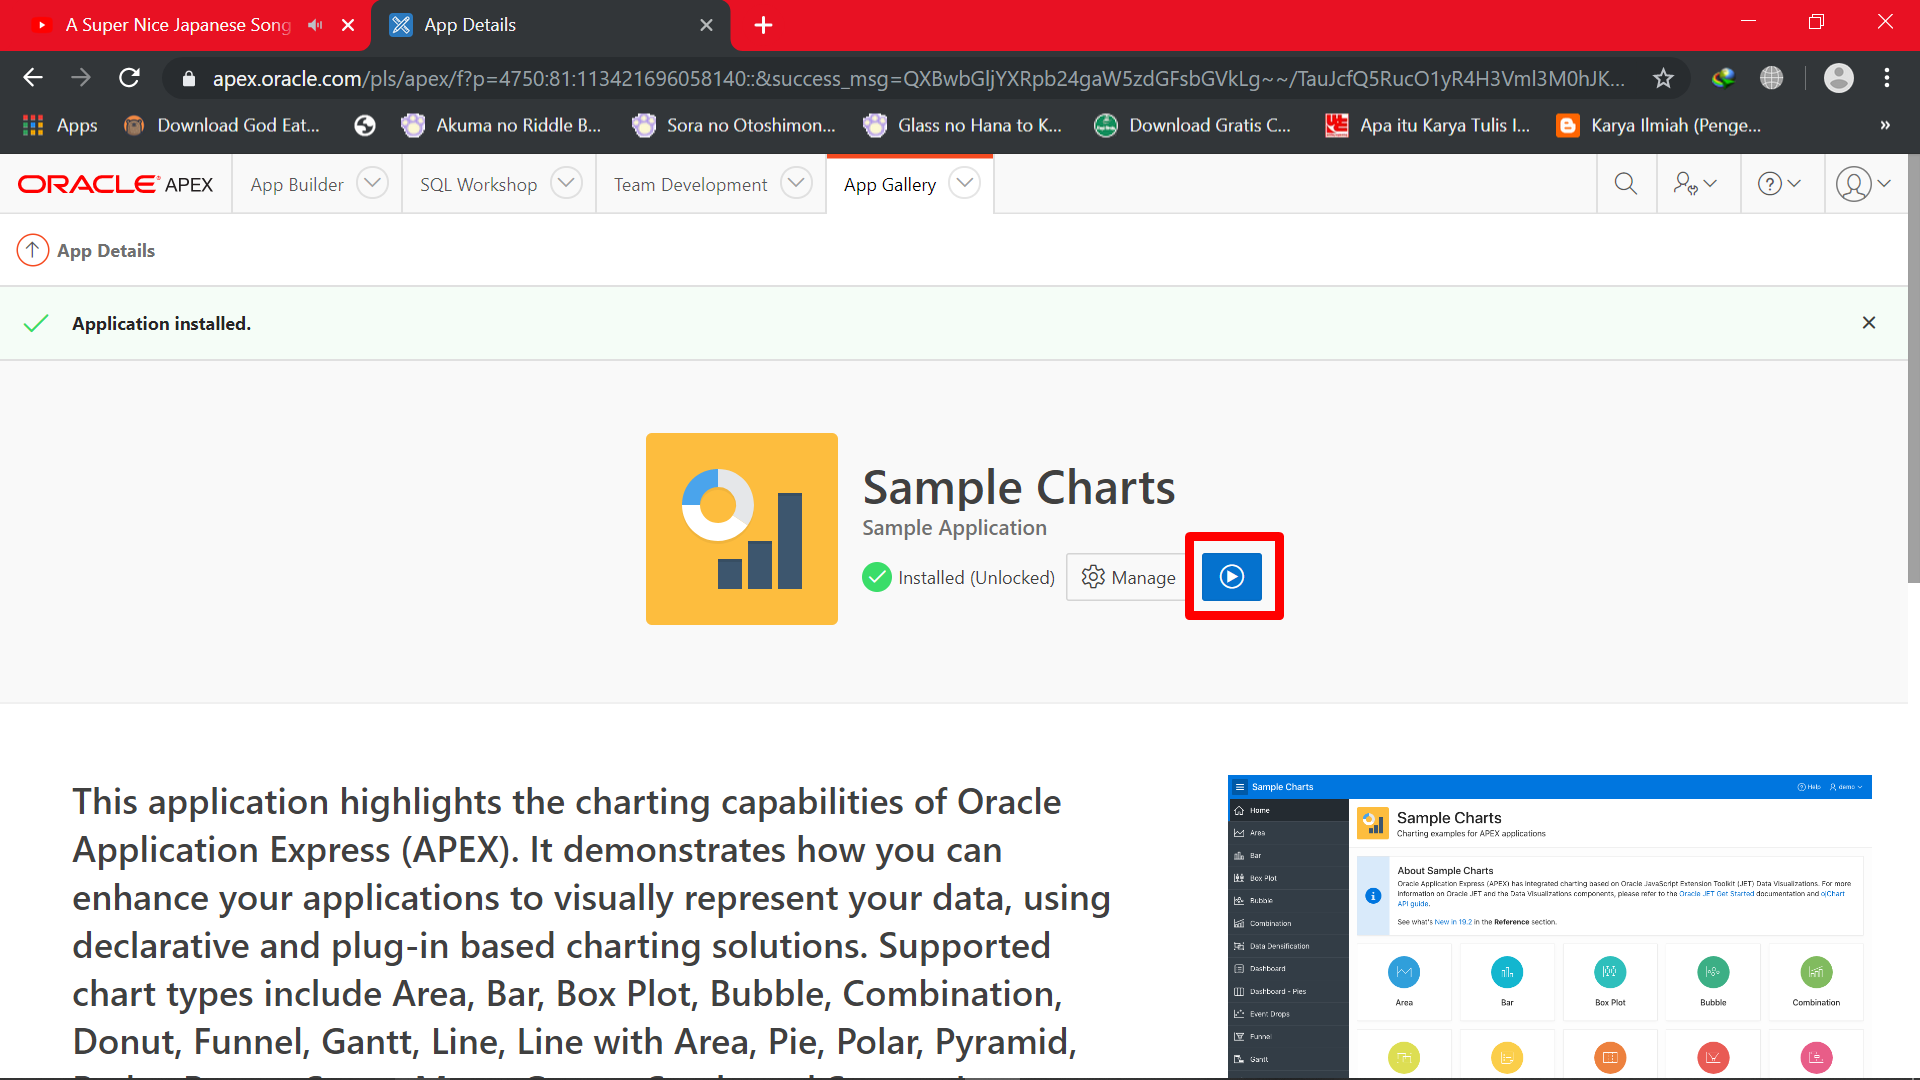
\includegraphics[width=12.5cm]{figures/Screenshot_30.png}
	\caption{App Gallery}
\end{figure}
\item Login ke Aplikasi dan akan masuk ke halaman utama Aplikasi Sample Charts.
\begin{figure}[!htpb]
	\centering
	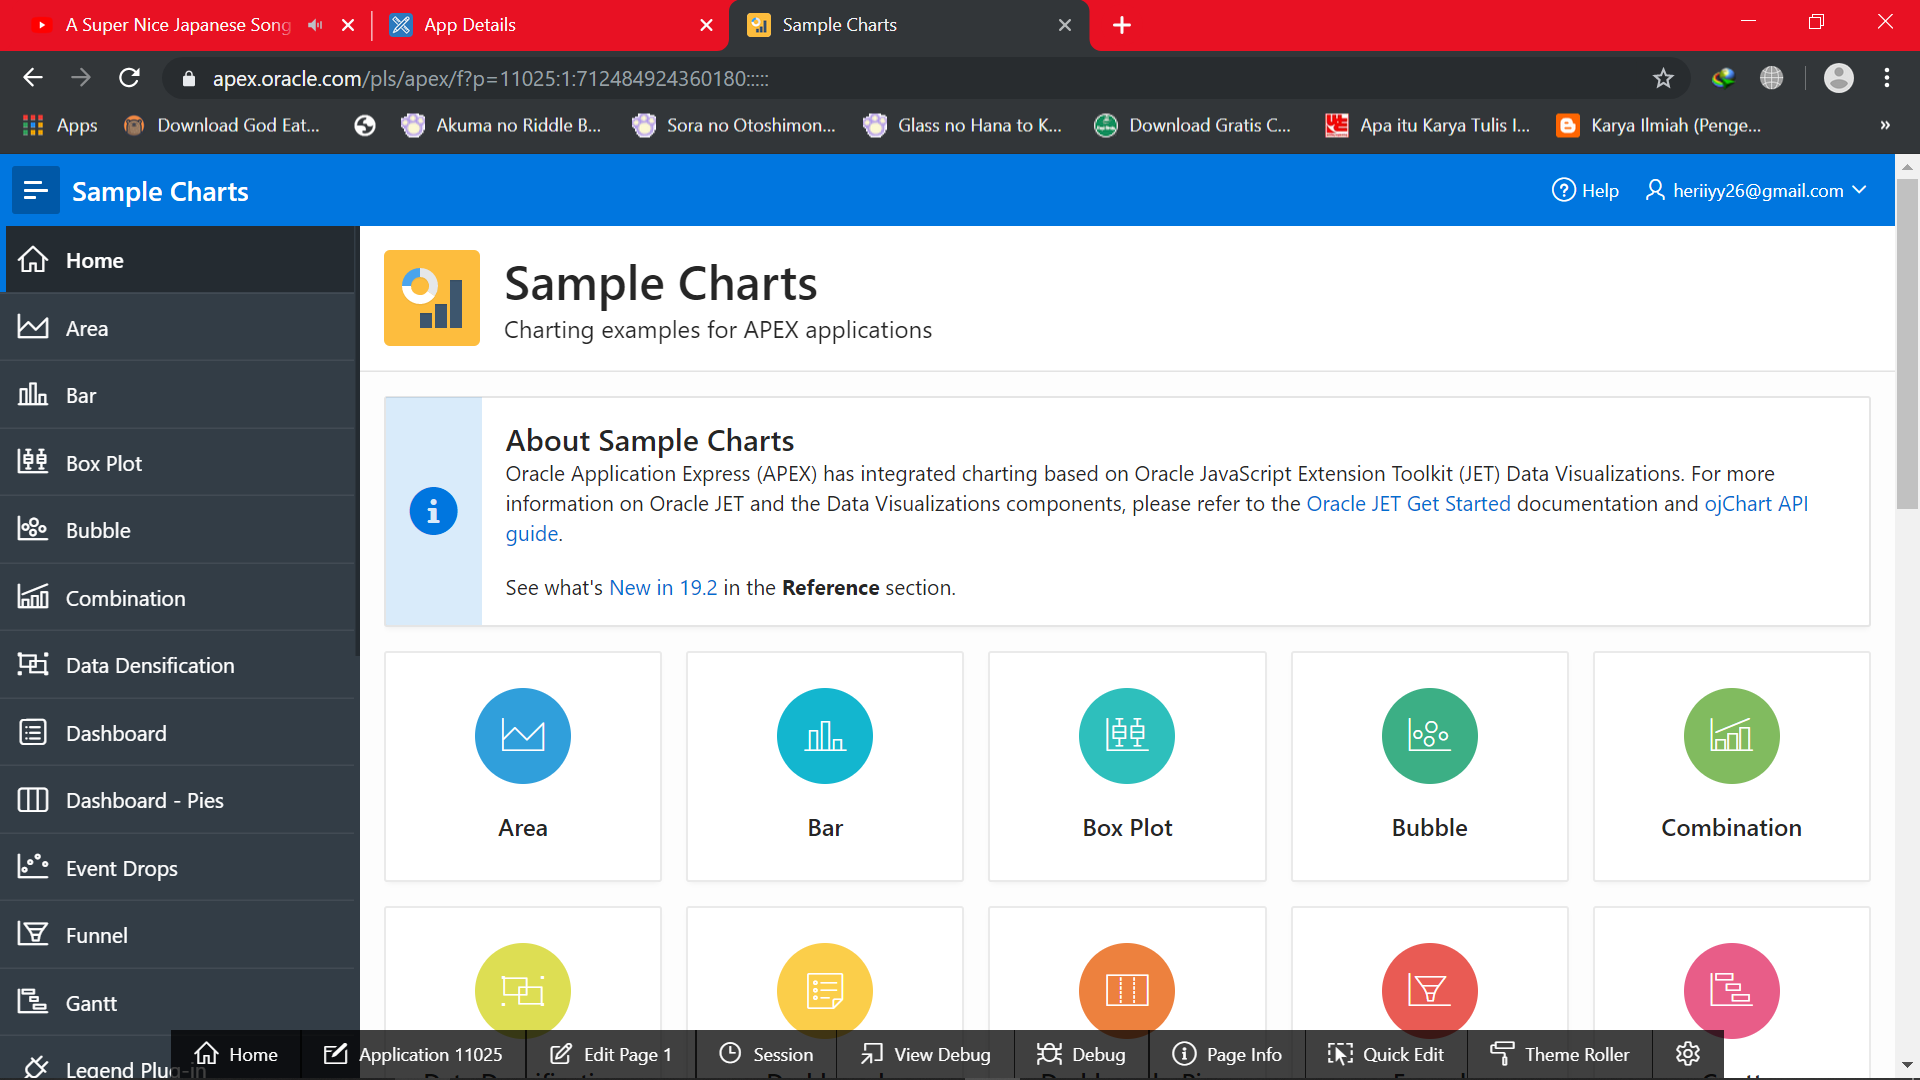
\includegraphics[width=12.5cm]{figures/Screenshot_31.png}
	\caption{App Gallery}
\end{figure}
\end{itemize}
\end{document}
